%%%%%%%%%%%%%%%%%%%%%%%%%%%%%%%%%%%%%%%%%%%%%%%%%%%%%%%%%%%%%%%%
%%%%%%%%%%%%%%%%%%%%%%%%%%%%%%%%%%%%%%%%%%%%%%%%%%%%%%%%%%%%%%%%
%%%%
%%%% This text file is part of the source of slides for
%%%% `Introduction to High-Performance Scientific Computing'
%%%% by Victor Eijkhout, copyright 2012
%%%%
%%%%%%%%%%%%%%%%%%%%%%%%%%%%%%%%%%%%%%%%%%%%%%%%%%%%%%%%%%%%%%%%
%%%%%%%%%%%%%%%%%%%%%%%%%%%%%%%%%%%%%%%%%%%%%%%%%%%%%%%%%%%%%%%%

\documentclass[headnav]{beamer}

\newenvironment{beamdisplayeq}%
 {\begin{equation}\small}{\end{equation}}

\usepackage{beamerthemeTACC}
\parskip=.5\baselineskip plus .5\baselineskip
\event{PCSE 2013}

\usepackage{graphicx,comment,multicol,undertilde}
\usepackage{hyperref}

\usepackage[algo2e]{algorithm2e}
\newenvironment{displayalgorithm}
 {\begin{algorithm2e}[H]}{\end{algorithm2e}}
\newenvironment{displayprocedure}[2]
 {\begin{procedure}[H]\caption{#1(#2)}}
 {\end{procedure}}

\def\sublocal{_{\mathrm\scriptstyle local}}
\newcommand\inv{^{-1}}
\usepackage{amsmath,arydshln,graphicx,comment,multicol,undertilde}
\newcommand\argmin{\mathop{\mathrm{argmin}}}
\newcommand\setspan[1]{[\![#1]\!]}

\begin{document}
\title{Parallelism in Applied Math Calculations}
\author{Victor Eijkhout}
\date{374/394 spring 2013}
\frame{\titlepage}

\frame{\frametitle{ODEs and PDEs}
Time-evolving phenomena:
IVP (Initial Value Problem), usually Ordinary Differential Equations

Space-constraint phenomena:
BVP (Boundary Value Problem), usually Partial Differential Equations

}

\sectionframe{Approximating Differential Equations}

\frame{\frametitle{Finite difference approximation}

  We turn the continuous problem into a discrete one, by looking at finite
  time/space steps.

  Assume all functions are sufficiently smooth, and use Taylor series:
  \[ u(t+\Delta t)=u(t)+u'(t)\Delta t+u''(t)\frac{\Delta t^2}{2!}
  + u'''(t)\frac{\Delta t^3}{3!}+\cdots \]
  This gives for $u'$:
  \[ u'(t) = \frac{u(t+\Delta t)-u(t)}{\Delta t}+O(\Delta t^2) \]
  So we approximate
  \[ u'(t)\approx \frac{u(t+\Delta t)-u(t)}{\Delta t} \]
  and the ``truncation error'' is $O(\Delta t^2)$.
}

\frame{\frametitle{Finite differences 2}

  How does this help? In $u'=f(t,u)$ substitute
  \[ u'(t)\rightarrow \frac{u(t+\Delta t)-u(t)}{\Delta t} \]
  giving
  \[ \frac{u(t+\Delta t)-u(t)}{\Delta t} = f(t,u(t)) \]
  or 
  \[ u(t+\Delta t) = u(t) + \Delta t\,f(t,u(t)) \]
  Let $t_0=0$, $t_{k+1}=t_k+\Delta t=\cdots=(k+1)\Delta t$, $u(t_k)=u_k$:
  \[ u_{k+1}=u_k+\Delta t\,f(t_k,u_k) \]
  Discretization\\`Explicit Euler' or `Euler forward'.

  Does this compute something close to the true solution?\\
  `Discretization error'
}

\frame{\frametitle{Boundary value problems}
  Consider $u''(x)=f(x,u,u')$ for $x\in[a,b]$ where $u(a)=u_a$, $u(b)=u_b$
in 1D and
\begin{equation}
 \hbox{$-u_{xx}(\bar x)-u_{yy}(\bar x)=f(\bar x)$ for
   $x\in\Omega=[0,1]^2$ 
    with $u(\bar x)=u_0$ on $\delta\Omega$.}
 \label{eq:2nd-order-bvp-2D}
 \end{equation}
in 2D.
}
\frame{\frametitle{Approximation of 2nd order derivatives}
\footnotesize
  Taylor series (write $h$ for $\delta x$):
  \[ u(x+h)=u(x)+u'(x)h+u''(x)\frac{h^2}{2!}+u'''(x)\frac{h^3}{3!}
  +u^{(4)}(x)\frac{h^4}{4!}+u^{(5)}(x)\frac{h^5}{5!}+\cdots \]
  and
  \[ u(x-h)=u(x)-u'(x)h+u''(x)\frac{h^2}{2!}-u'''(x)\frac{h^3}{3!}
  +u^{(4)}(x)\frac{h^4}{4!}-u^{(5)}(x)\frac{h^5}{5!}+\cdots \]
  Subtract:
  \[ u(x+h)+u(x-h)=2u(x)+u''(x)h^2+u^{(4)}(x)\frac{h^4}{12}+\cdots \]
  so
  \[ u''(x)=\frac{u(x+h)-2u(x)+u(x-h)}{h^2}-u^{(4)}(x)\frac{h^4}{12}+\cdots \]


  Numerical scheme:
  \[ -\frac{u(x+h)-2u(x)+u(x-h)}{h^2}=f(x,u(x),u'(x)) \]
  (2nd order PDEs are very common!)
}

\frame{\frametitle{This leads to linear algebra}
  \[ -\frac{u(x+h)-2u(x)+u(x-h)}{h^2}=f(x,u(x),u'(x)) \]
  Equally spaced points on $[0,1]$: $x_k=kh$ where $h=1/n$, then
  \[ -u_{k+1}+2u_k-u_{k-1} = h^2\,f(x_k,u_k,u'_k)
  \quad\hbox{for $k=1,\ldots,n-1$} \]
  Written as matrix equation:
  \[
  \left(
    \begin{matrix}
      2&-1\\ -1&2&-1\\ &\ddots&\ddots&\ddots
    \end{matrix}\right)
  \left(
    \begin{matrix}
      u_1\\ u_2\\ \vdots
    \end{matrix}\right)
  = 
  \left(
    \begin{matrix}
      h^2f_1+u_0\\ h^2f_2\\ \vdots
    \end{matrix}\right)
  \]
}

\frame{\frametitle{Matrix properties}

  \begin{itemize}
  \item Very sparse, banded
  \item Symmetric (only because 2nd order problem)
  \item Sign pattern: positive diagonal, nonpositive off-diagonal\\
    (true for many second order methods)
  \item Positive definite (just like the continuous problem)
  \end{itemize}
}

\frame{\frametitle{Initial Boundary value problem}
  Heat conduction in a rod $T(x,t)$ for $x\in[a,b]$, $t>0$:
  \[ \frac\partial{\partial t}T(x,t)-\alpha\frac{\partial^2}{\partial x^2}T(x,t)
  =q(x,t) \]
  \begin{itemize}
  \item Initial condition: $T(x,0)=T_0(x)$
  \item Boundary conditions: $T(a,t)=T_a(t)$, $T(b,t)=T_b(t)$
  \item Material property: $\alpha>0$ is thermal diffusivity
  \item Forcing function: $q(x,t)$ is externally applied heating.
  \end{itemize}
  The equation $u''(x)=f$ above is the steady state.
}

\frame{\frametitle{Discretization}
  Space discretization: $x_0=a$, $x_n=b$, $x_{j+1}=x_j+\Delta x$\\
  Time discretiation: $t_0=0$, $t_{k+1}=t_k+\Delta t$\\
  Let $T^k_j$ approximate $T(x_j,t_k)$

  Space:
  \[ \frac\partial{\partial t}T(x_j,t)-\alpha
  \frac{T(x_{j-1},t)-2T(x_j,t)+T(x_{j+1},t)}{\Delta x^2}=q(x_j,t) \]
  Explicit time stepping:
  \[ \frac{T_j^{k+1}-T_j^k}{\Delta t}-\alpha
  \frac{T_{j-1}^k-2T_j^k+T_{j+1}^k}{\Delta x^2}=q_j^k \]
  Implicit time stepping:
  \[ \frac{T_j^{k+1}-T_j^k}{\Delta t}-\alpha
  \frac{T_{j-1}^{k+1}-2T_j^{k+1}+T_{j+1}^{k+1}}{\Delta x^2}=q_j^{k+1} \]
}

\frame{\frametitle{Computational form:   explicit}
  \[ T_j^{k+1}=T_j^k+\frac{\alpha\Delta t}{\Delta x^2}
  (T_{j-1}^k-2T_j^k+T_{j+1}^k)+\Delta t q_j^k \]
  This has an explicit form:
  \[ \utilde T^{k+1}=\left(I+\frac{\alpha\Delta t}{\Delta x^2}K\right
  )\utilde T^k+\Delta t\utilde q^k \]
where $K$ is the Laplace matrix
}

\frame{\frametitle{Computational form: implicit}
  \[ T_j^{k+1}-\frac{\alpha\Delta t}{\Delta x^2}
  (T_{j-1}^k-2T_j^k+T_{j+1}^k)=T_j^k+\Delta t q_j^k \]
  This has an implicit form:
  \[ \left(I-\frac{\alpha\Delta t}{\Delta x^2}K\right)\utilde T^{k+1}=
  \utilde T^k+\Delta t\utilde q^k \]
  Needs to solve a linear system in every time step
}
\def\fr{\frac{\alpha\Delta t}{\Delta x^2}}

\frame{\frametitle{Stability of explicit scheme}
Needs
    \[ \Delta t<\frac{\Delta x^2}{2\alpha} \]
    big restriction on size of time steps
}

\frame{\frametitle{Stability of implicit scheme}
Stability condition always satisfied:
  method always stable.
}

\frame{\frametitle{Sparse matrix in 2D case}
Sparse matrices so far were tridiagonal: only in 1D case.

Two-dimensional: $-u_{xx}-u_{yy}=f$ on unit square $[0,1]^2$

Difference equation: {\small $4u(x,y)-u(x+h,y)-u(x-h,y)-u(x,y+h)-u(x,y-h)=h^2f(x,y)$}

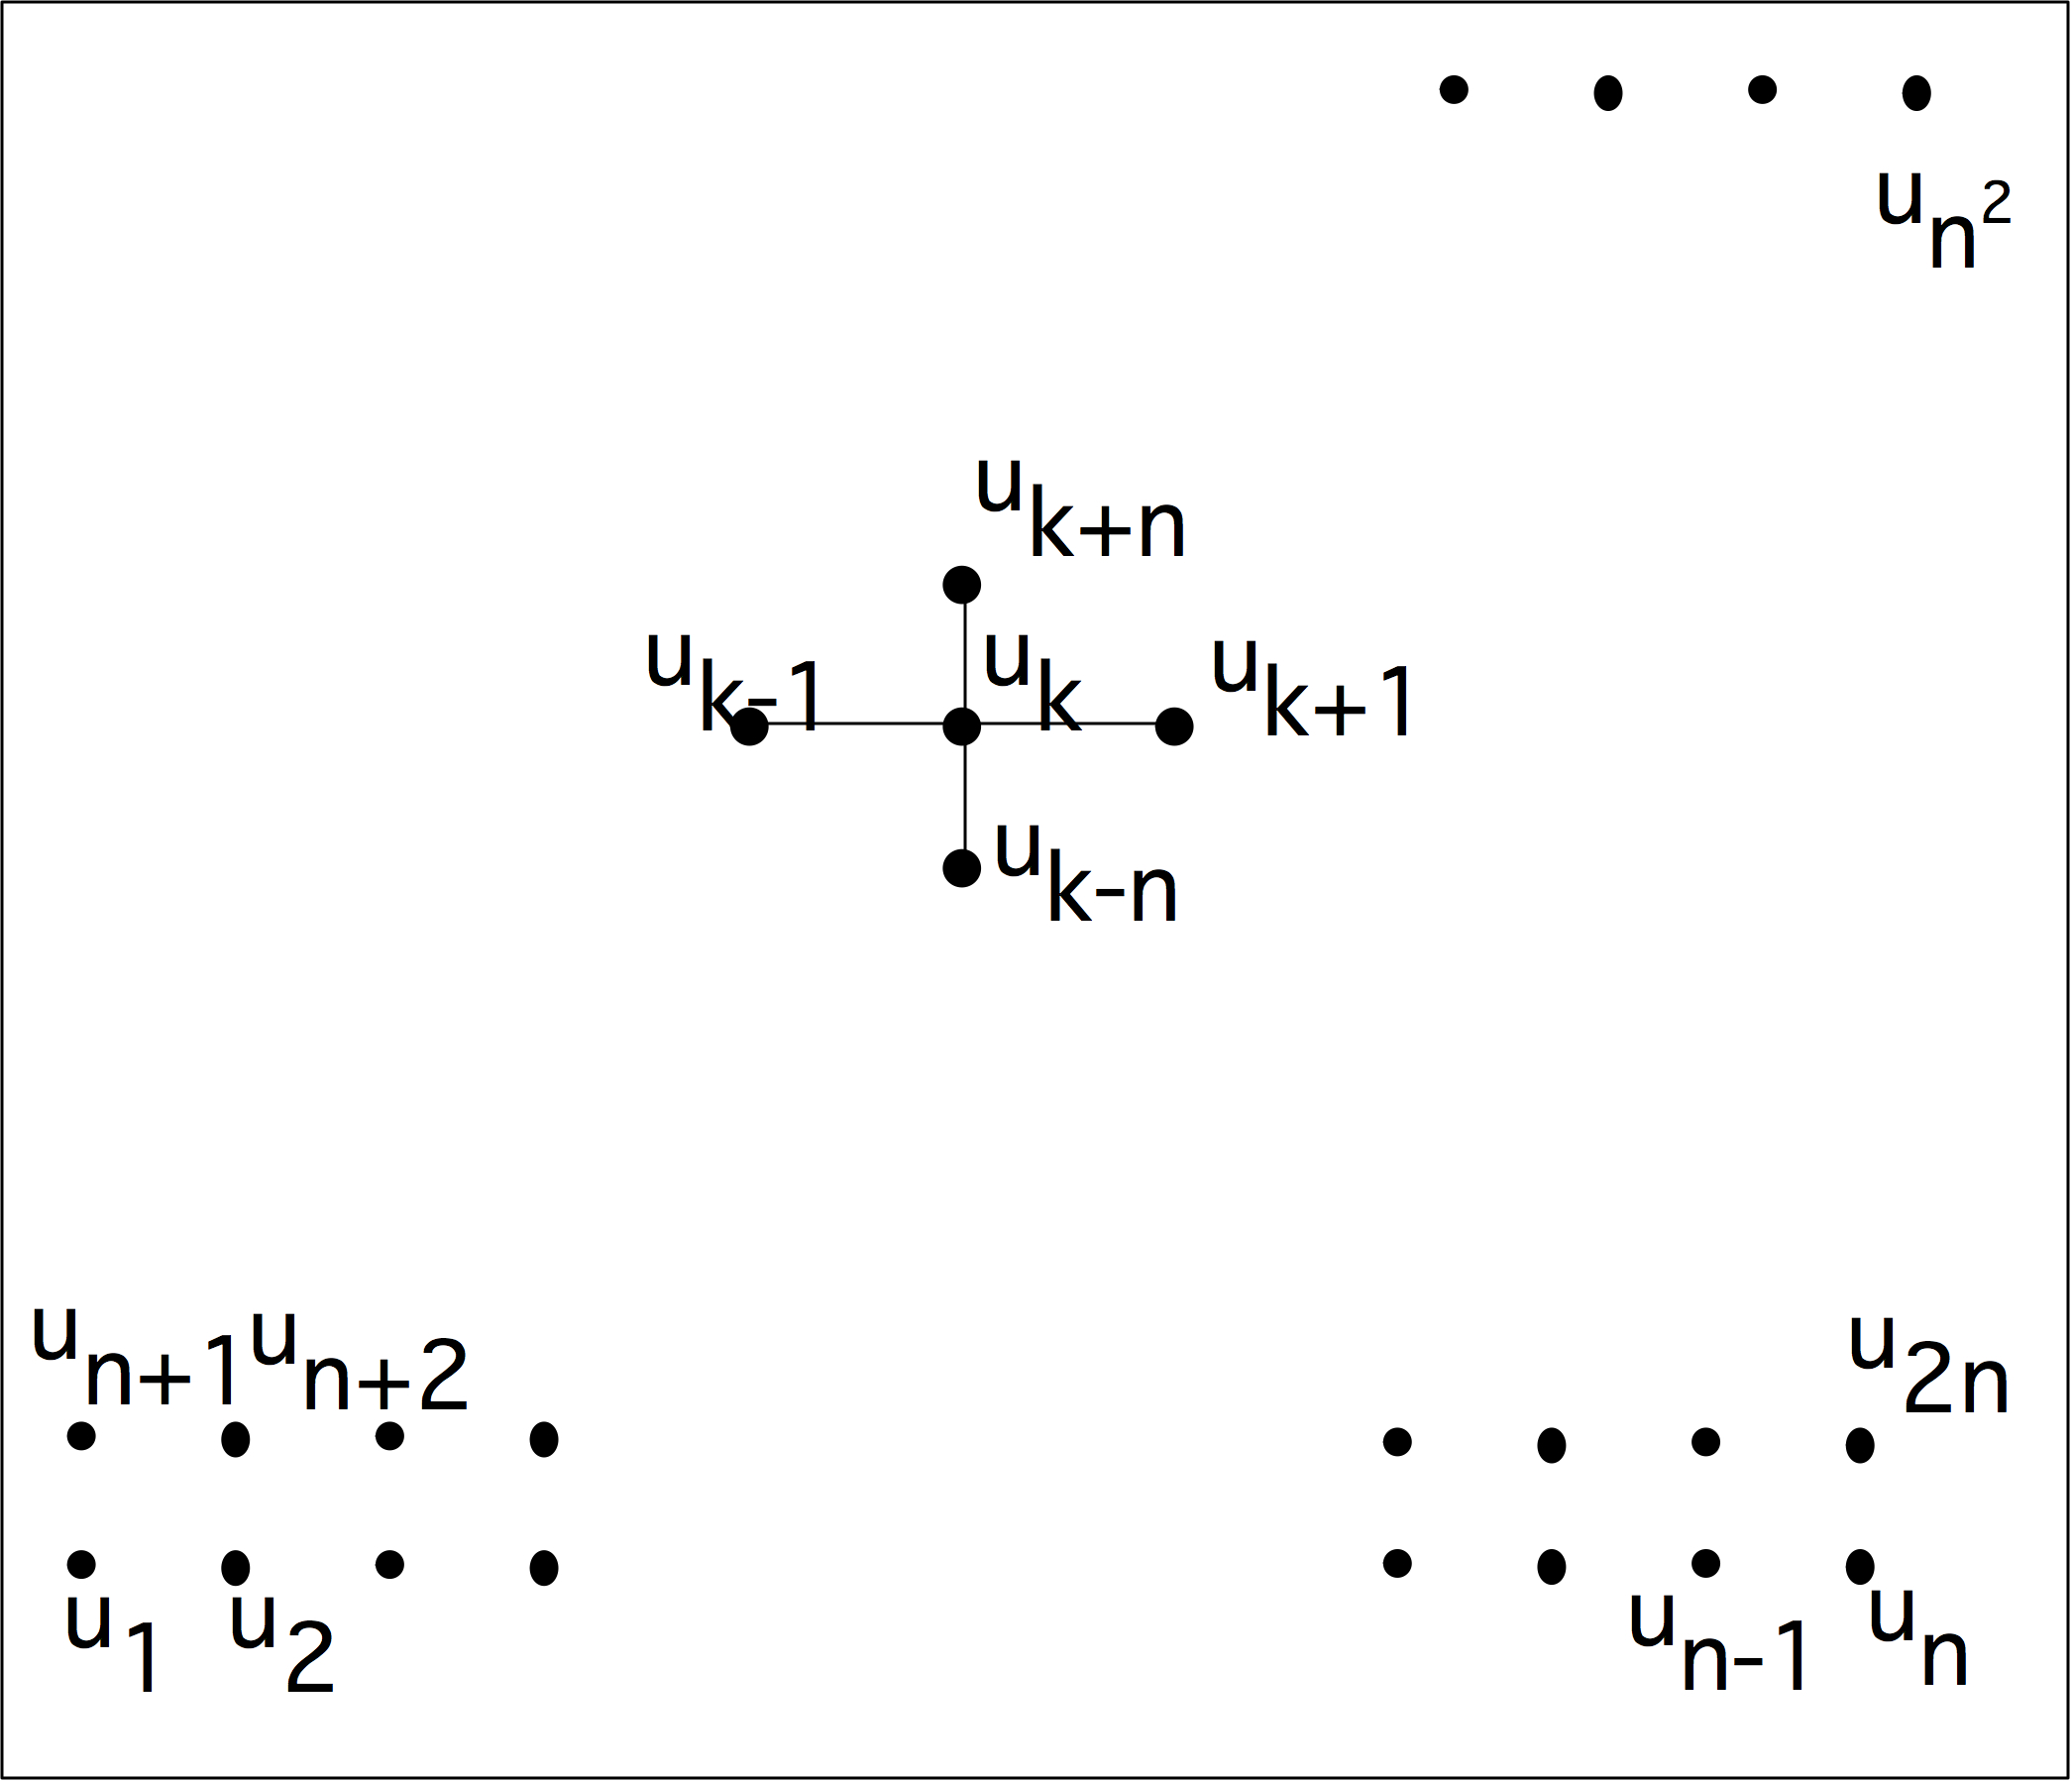
\includegraphics[scale=.07]{graphics/laplacedomain}
}

\frame{\frametitle{Graph theory of sparse matrices}
  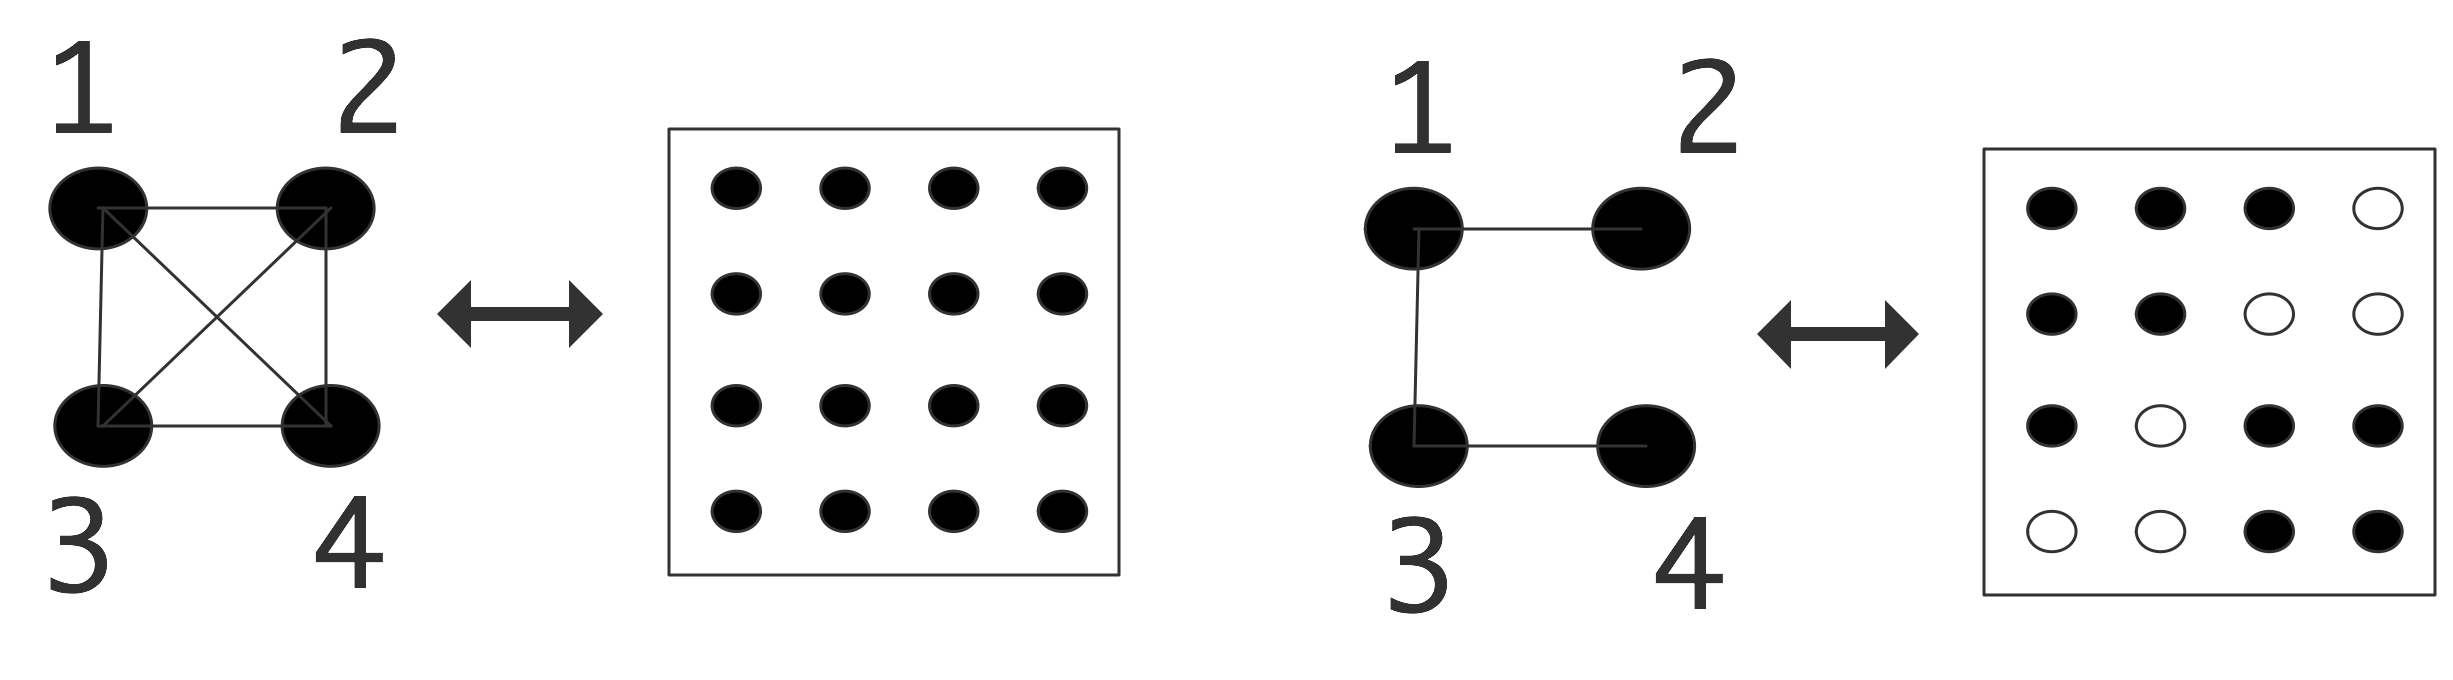
\includegraphics[scale=.12]{graphics/matrix-graph}
}

\frame{\frametitle{The graph view of things}
Poisson eq:
\[ 4u_k-u_{k-1}-u_{k+1}-u_{k-n}-u_{k+n}=f_k \]
Consider a graph where $\{u_k\}_k$ are the edges\\
and $(u_i,u_j)$ is an edge iff $a_{ij}\not=0$.

This is the (adjacency) graph of a sparse matrix.
}

\frame{\frametitle{Sparse matrix from 2D equation}
\small
\[
  \left(\begin{array}{ccccc|ccccc|cc}
    4&-1&&&\emptyset&-1&&&&\emptyset&\\ 
    -1&4&1&&&&-1&&&&\\ 
    &\ddots&\ddots&\ddots&&&&\ddots&&\\ 
    &&\ddots&\ddots&-1&&&&\ddots&\\ 
    \emptyset&&&-1&4&\emptyset&&&&-1&\\ \hline
    -1&&&&\emptyset&4&-1&&&&-1\\
    &-1      &      &&&-1      &4       &-1      &&&&-1\\
    &\uparrow&\ddots&&&\uparrow&\uparrow&\uparrow&&  &&\uparrow\\
    &k-n     &      &&&k-1     &k       &k+1     &&-1&&k+n\\
    &&&&-1&&&&-1&4&&\\ \hline
    &        &      &&&\ddots  &        &        &&  &\ddots\\
  \end{array}\right)
\]
}

\frame{\frametitle{Matrix properties}

  \begin{itemize}
  \item Very sparse, banded
  \item Symmetric (only because 2nd order problem)
  \item Sign pattern: positive diagonal, nonpositive off-diagonal\\
    (true for many second order methods)
  \item Positive definite (just like the continuous problem)
  \item Constant diagonals: only because of the constant coefficient
    differential equation
  \end{itemize}
}

\frame{\frametitle{Realistic meshes}
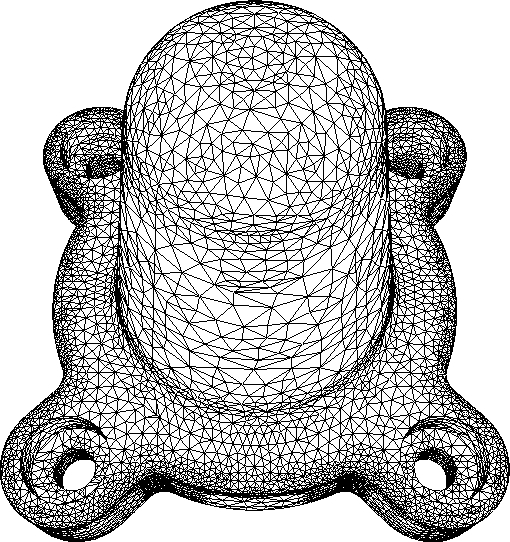
\includegraphics[scale=.3]{graphics/img206}
}

\sectionframe{Iterative solution methods}
\input iterative

\sectionframe{Sparse matrix-vector product}

\frame{\frametitle{Sparse matrix storage}

 Matrix above has many zeros: $n^2$ elements but only $O(n)$
  nonzeros. Big waste of space to store this as square array.

 Matrix is called  `sparse' if there are enough zeros to make
  specialized storage feasible.

  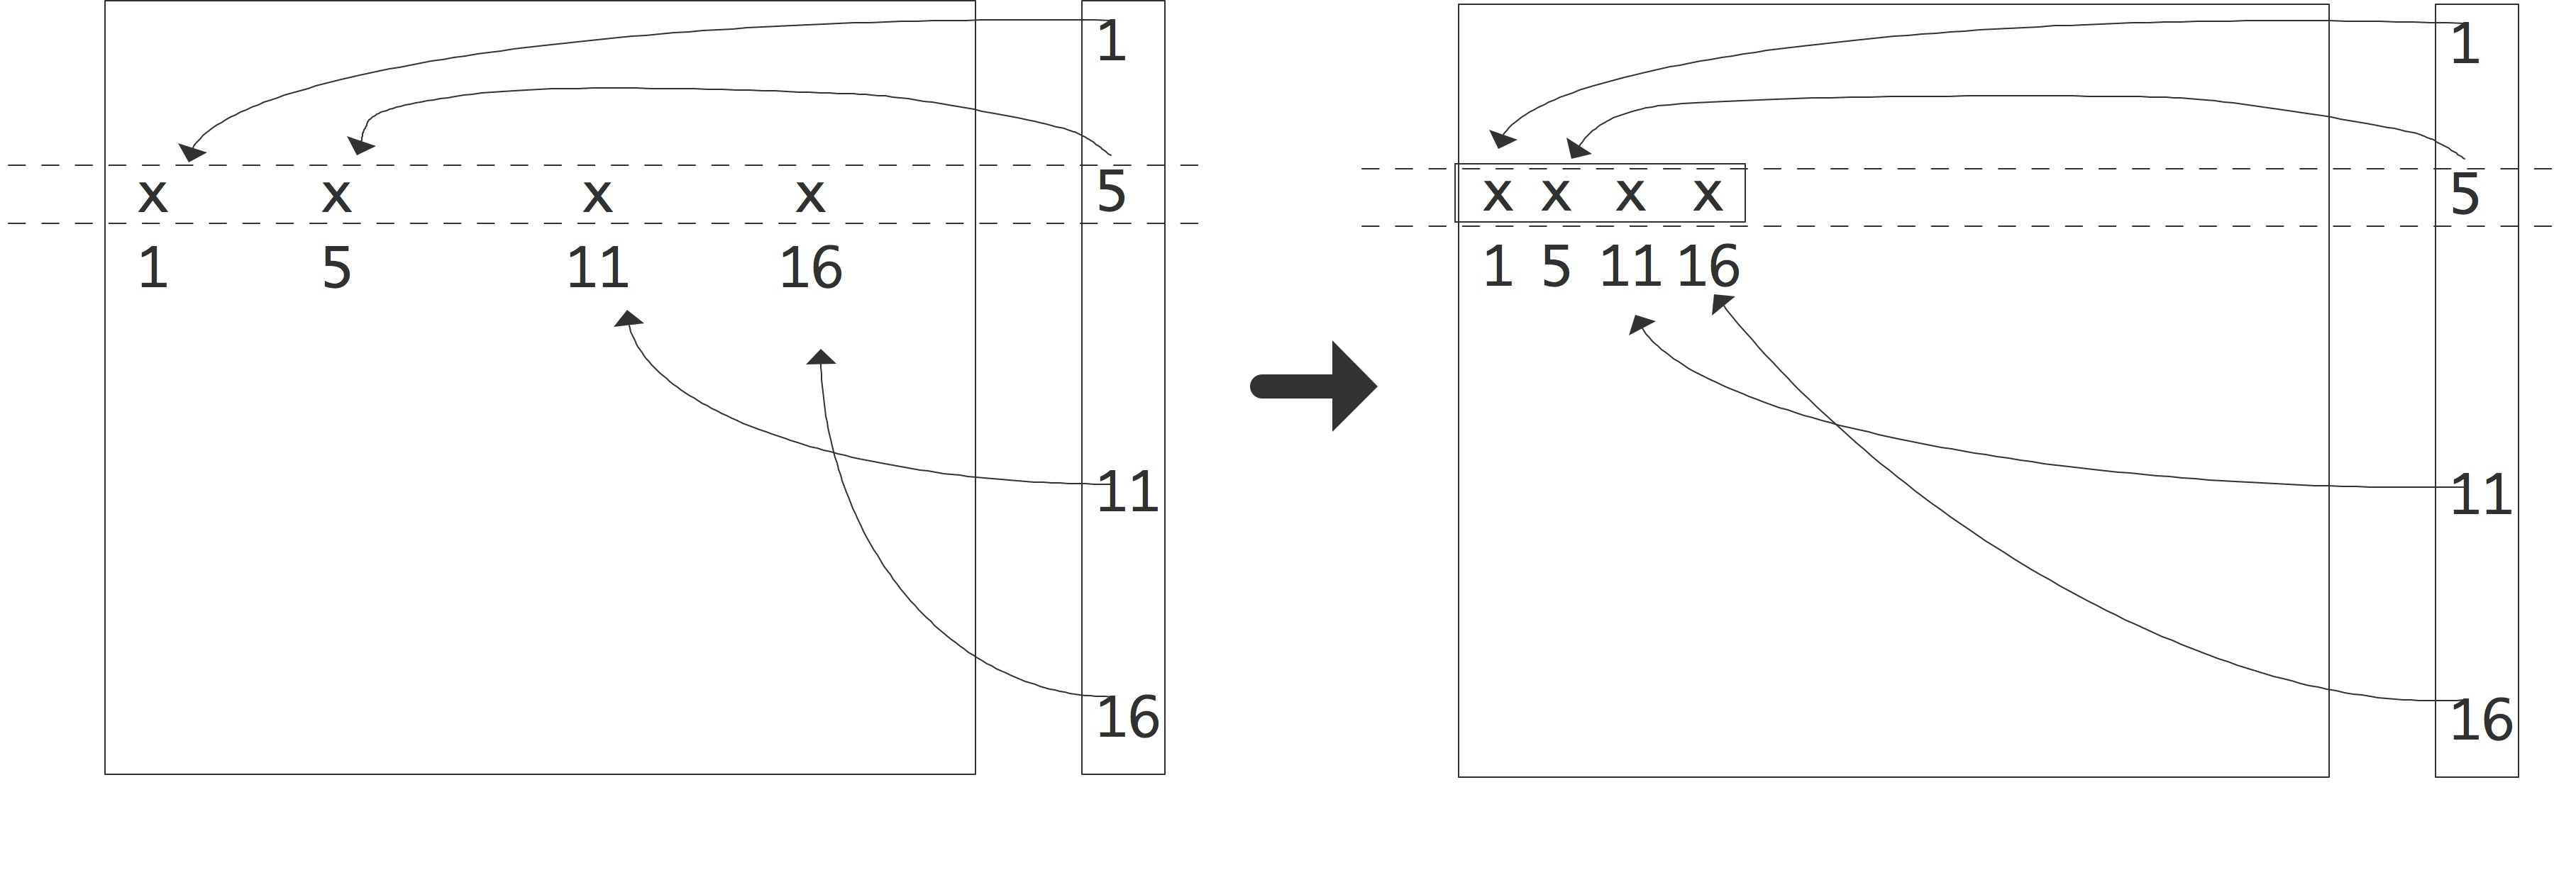
\includegraphics[scale=.08]{graphics/crs}
}

\frame{\frametitle{Compressed Row Storage}
\begin{equation}
A =
\left(\begin{array}{rrrrrr}
      10 &  0 &  0 & 0  &-2 &  0 \\
       3 &  9 &  0 & 0  & 0 &  3 \\
       0 &  7 &  8 & 7  & 0 &  0 \\
       3 &  0 &  8 & 7  & 5 &  0 \\
       0 &  8 &  0 & 9  & 9 & 13 \\
       0 &  4 &  0 & 0  & 2 & -1
           \end{array}
\right) ~.
\end{equation}
 Compressed Row Storage (CRS): store all nonzeros by row, their column
  indices, pointers to where the columns start (1-based indexing):
\begin{center}
\begin{tabular}{|r|r|r|r|r|r|r|r|r|r|r|r|r|r|r|r|} \hline
{\tt val}     &10 &-2& 3& 9& 3& 7& 8& 7& 3 $\cdots$  9&13& 4& 2&-1 \\ \hline
{\tt col\_ind}& 1 & 5& 1& 2& 6& 2& 3& 4& 1 $\cdots$  5& 6& 2& 5& 6 \\ \hline
\end{tabular} \\
\vspace{.02 in}
\begin{tabular}{|r|r|r|r|r|r|r|r|} \hline
{\tt row\_ptr}& 1 & 3 & 6 & 9 & 13 & 17 & 20  \\ \hline
\end{tabular} ~.
\end{center}
}

\frame[containsverbatim]{\frametitle{Sparse matrix operations}

  Most common operation: matrix-vector product
\begin{verbatim}
for (row=0; row<nrows; row++) {
   s = 0;
   for (icol=ptr[row]; icol<ptr[row+1]; icol++) {
      int col = ind[icol];
      s += a[aptr] * x[col];
      aptr++;
   }
   y[row] = s;
}
\end{verbatim}
Operations with changes to the nonzero structure are much harder!

Locality?
}

\frame[containsverbatim]{\frametitle{Sparse matrix operations}

  Most common operation: matrix-vector product
\begin{verbatim}
for (row=0; row<nrows; row++) {
   s = 0;
   for (icol=ptr[row]; icol<ptr[row+1]; icol++) {
      int col = ind[icol];
      s += a[aptr] * x[col];
      aptr++;
   }
   y[row] = s;
}
\end{verbatim}
Operations with changes to the nonzero structure are much harder!

Indirect addressing of \texttt{x} gives low spatial and temporal locality.
}

\frame{\frametitle{Parallel matrix-vector product}
  \begin{itemize}
  \item Assume a division by block rows
  \item Every processor $p$ has a set of row indices $I_p$
  \end{itemize}
  Mvp on processor $p$: \[ \forall_i\colon y_i=\sum_j a_{ij}x_j \]
  \[ \forall_i\colon y_i=\sum_q\sum_{j\in I_q} a_{ij}x_j \]
}

\frame{\frametitle{}
Local and remote parts:

  \[ \forall_i\colon y_i=\sum_{j\in
    I_p}a_{ij}x_j+\sum_{q\not=p}\sum_{j\in I_q} a_{ij}x_j 
  \]
  Local part $I_p$ can be executed right away, $I_q$ requires
  communication.

  Combine:
  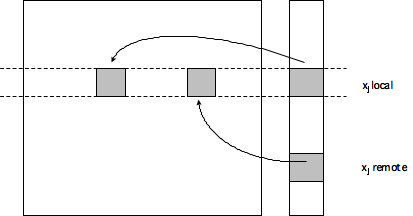
\includegraphics[scale=.6]{graphics/distmvp}
}

\frame{\frametitle{Sparse matrix-vector product}
Difference stencil

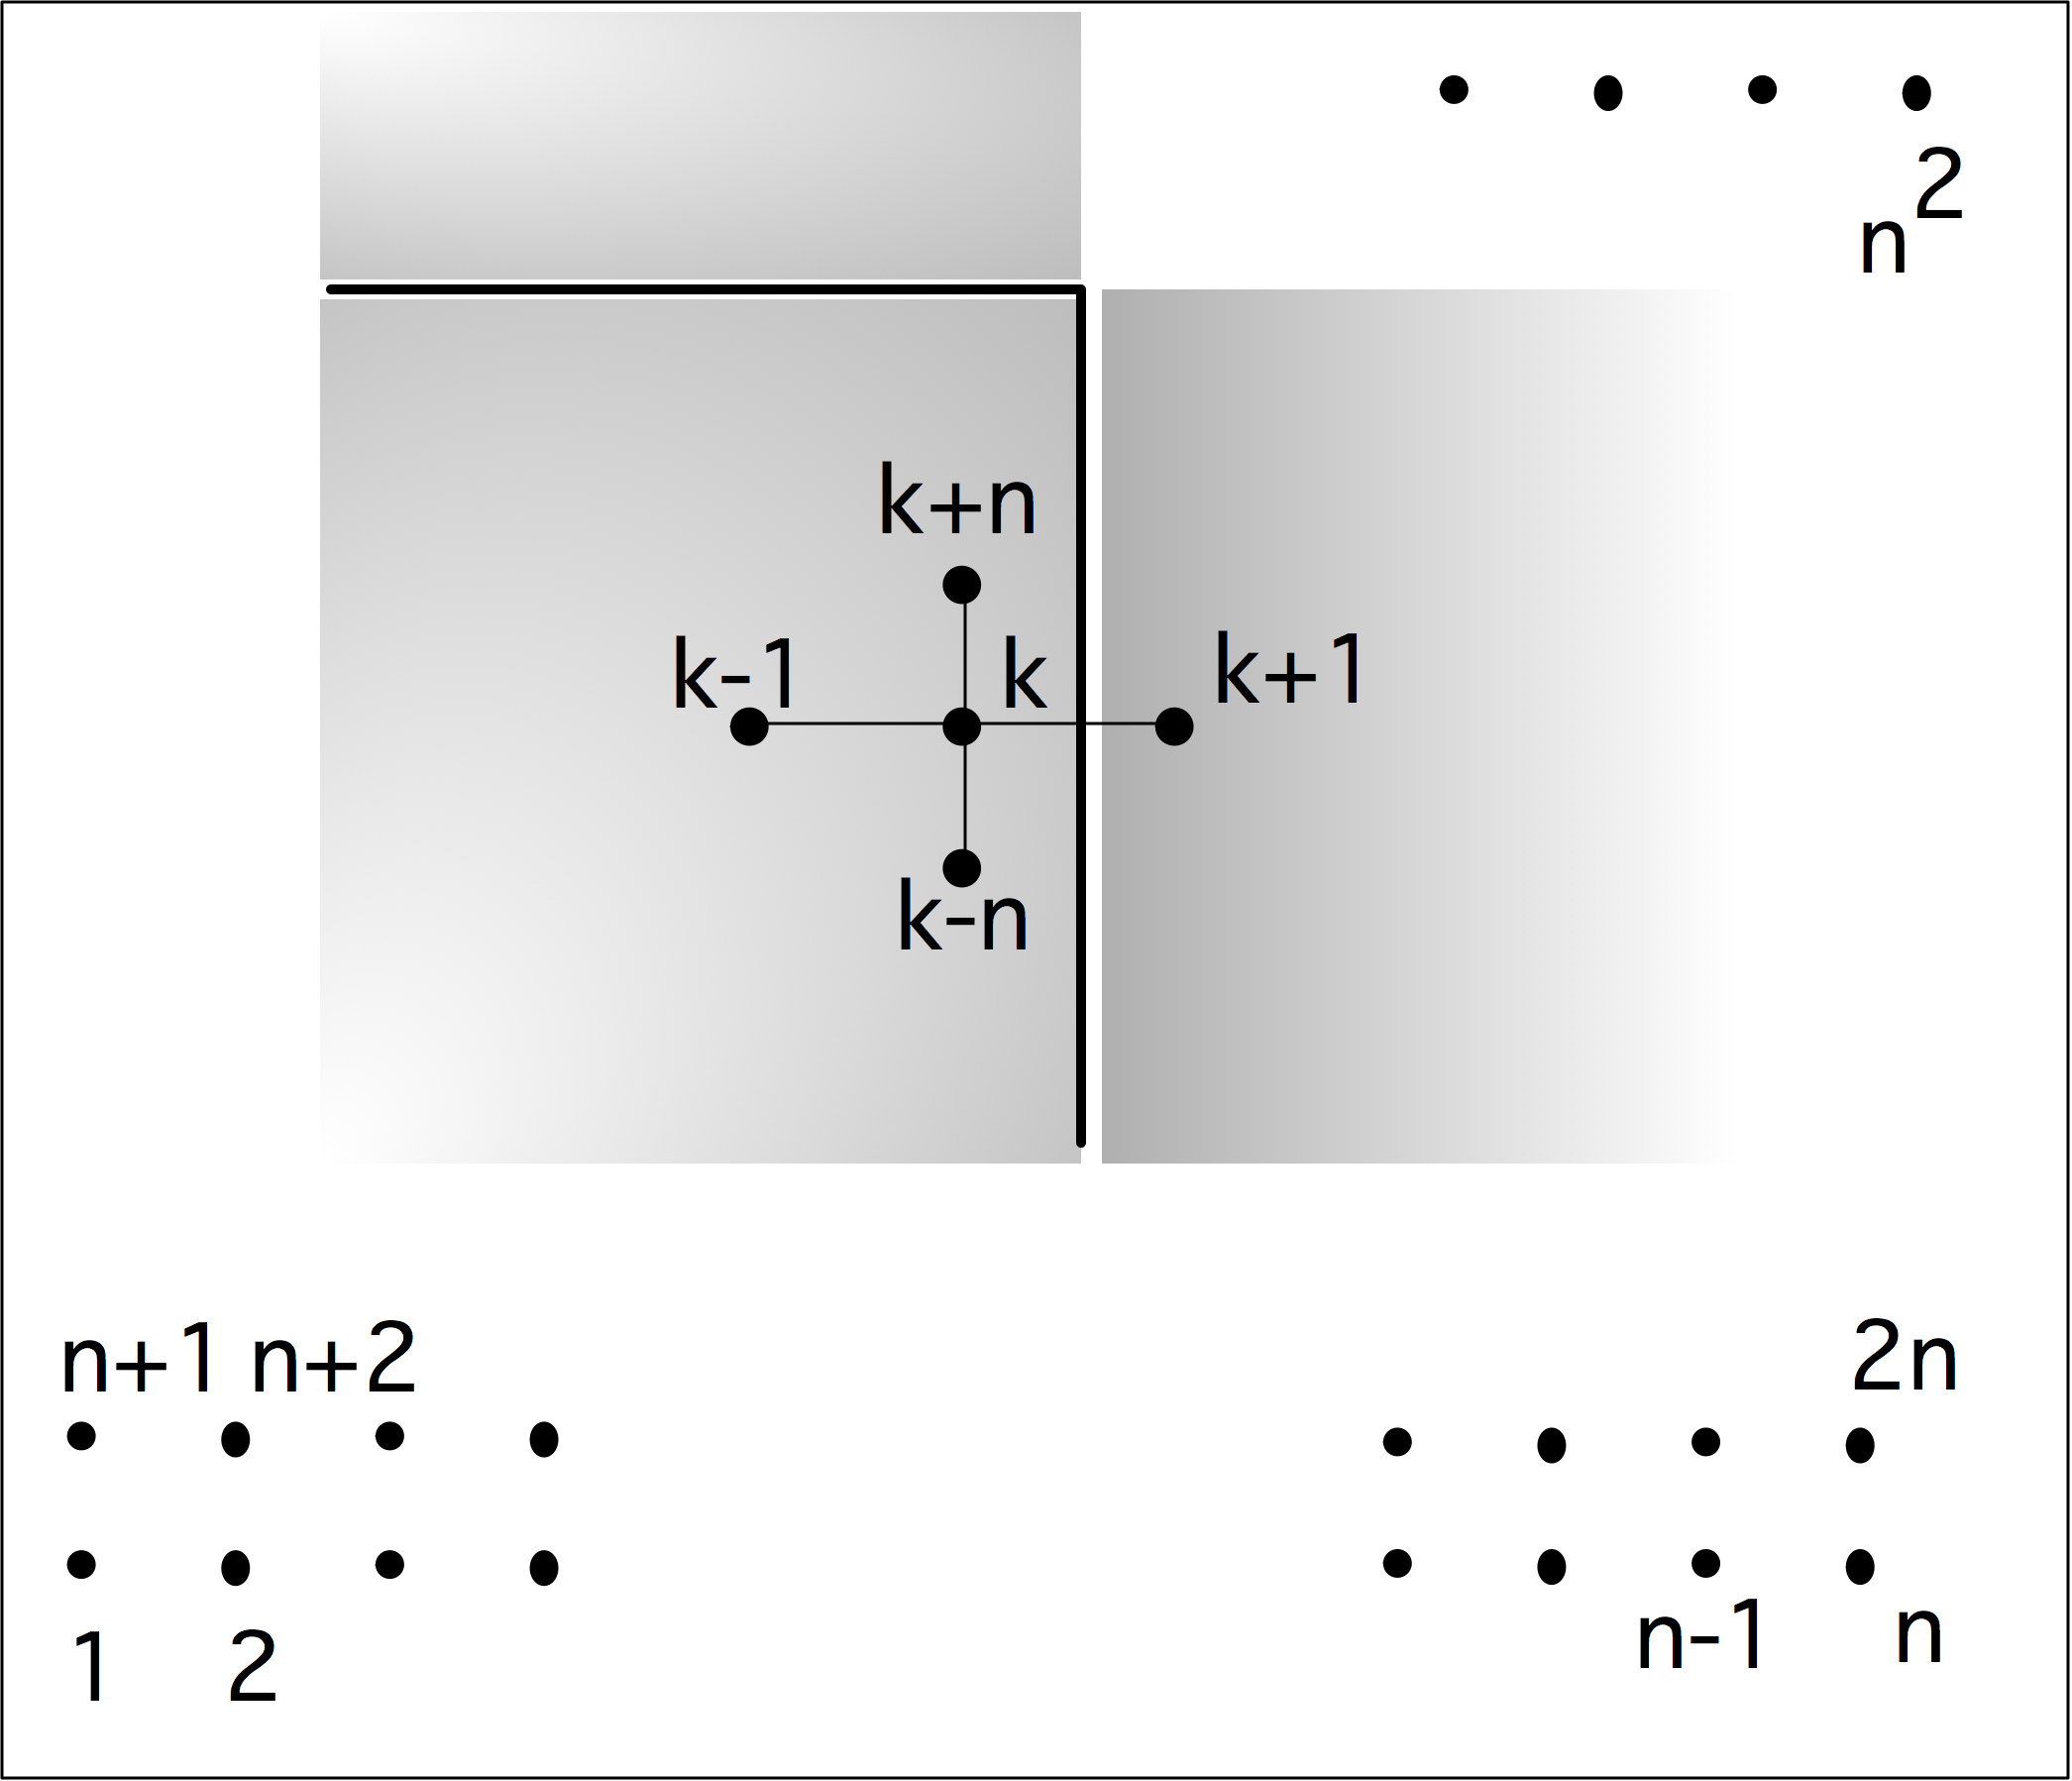
\includegraphics[scale=.1]{graphics/laplaceparallel}

}

\frame{\frametitle{}
induces ghost region:

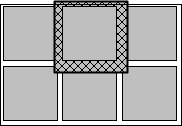
\includegraphics[scale=.7]{graphics/ghost}

Limited number of neighbours, limited buffer space
}

\frame{\frametitle{Scaling}
Separately 1D and 2D partitioning of the domain.
}
\frame{\frametitle{MPI Implementation}

}

\sectionframe{Gaussian elimination}

\frame{\frametitle{Differences between product and solving}
  \begin{itemize}
  \item Treatment of sparsity
  \item Operation count
  \item Ease of parallelizing
  \end{itemize}
}

\frame{\frametitle{Domain decomposition}
    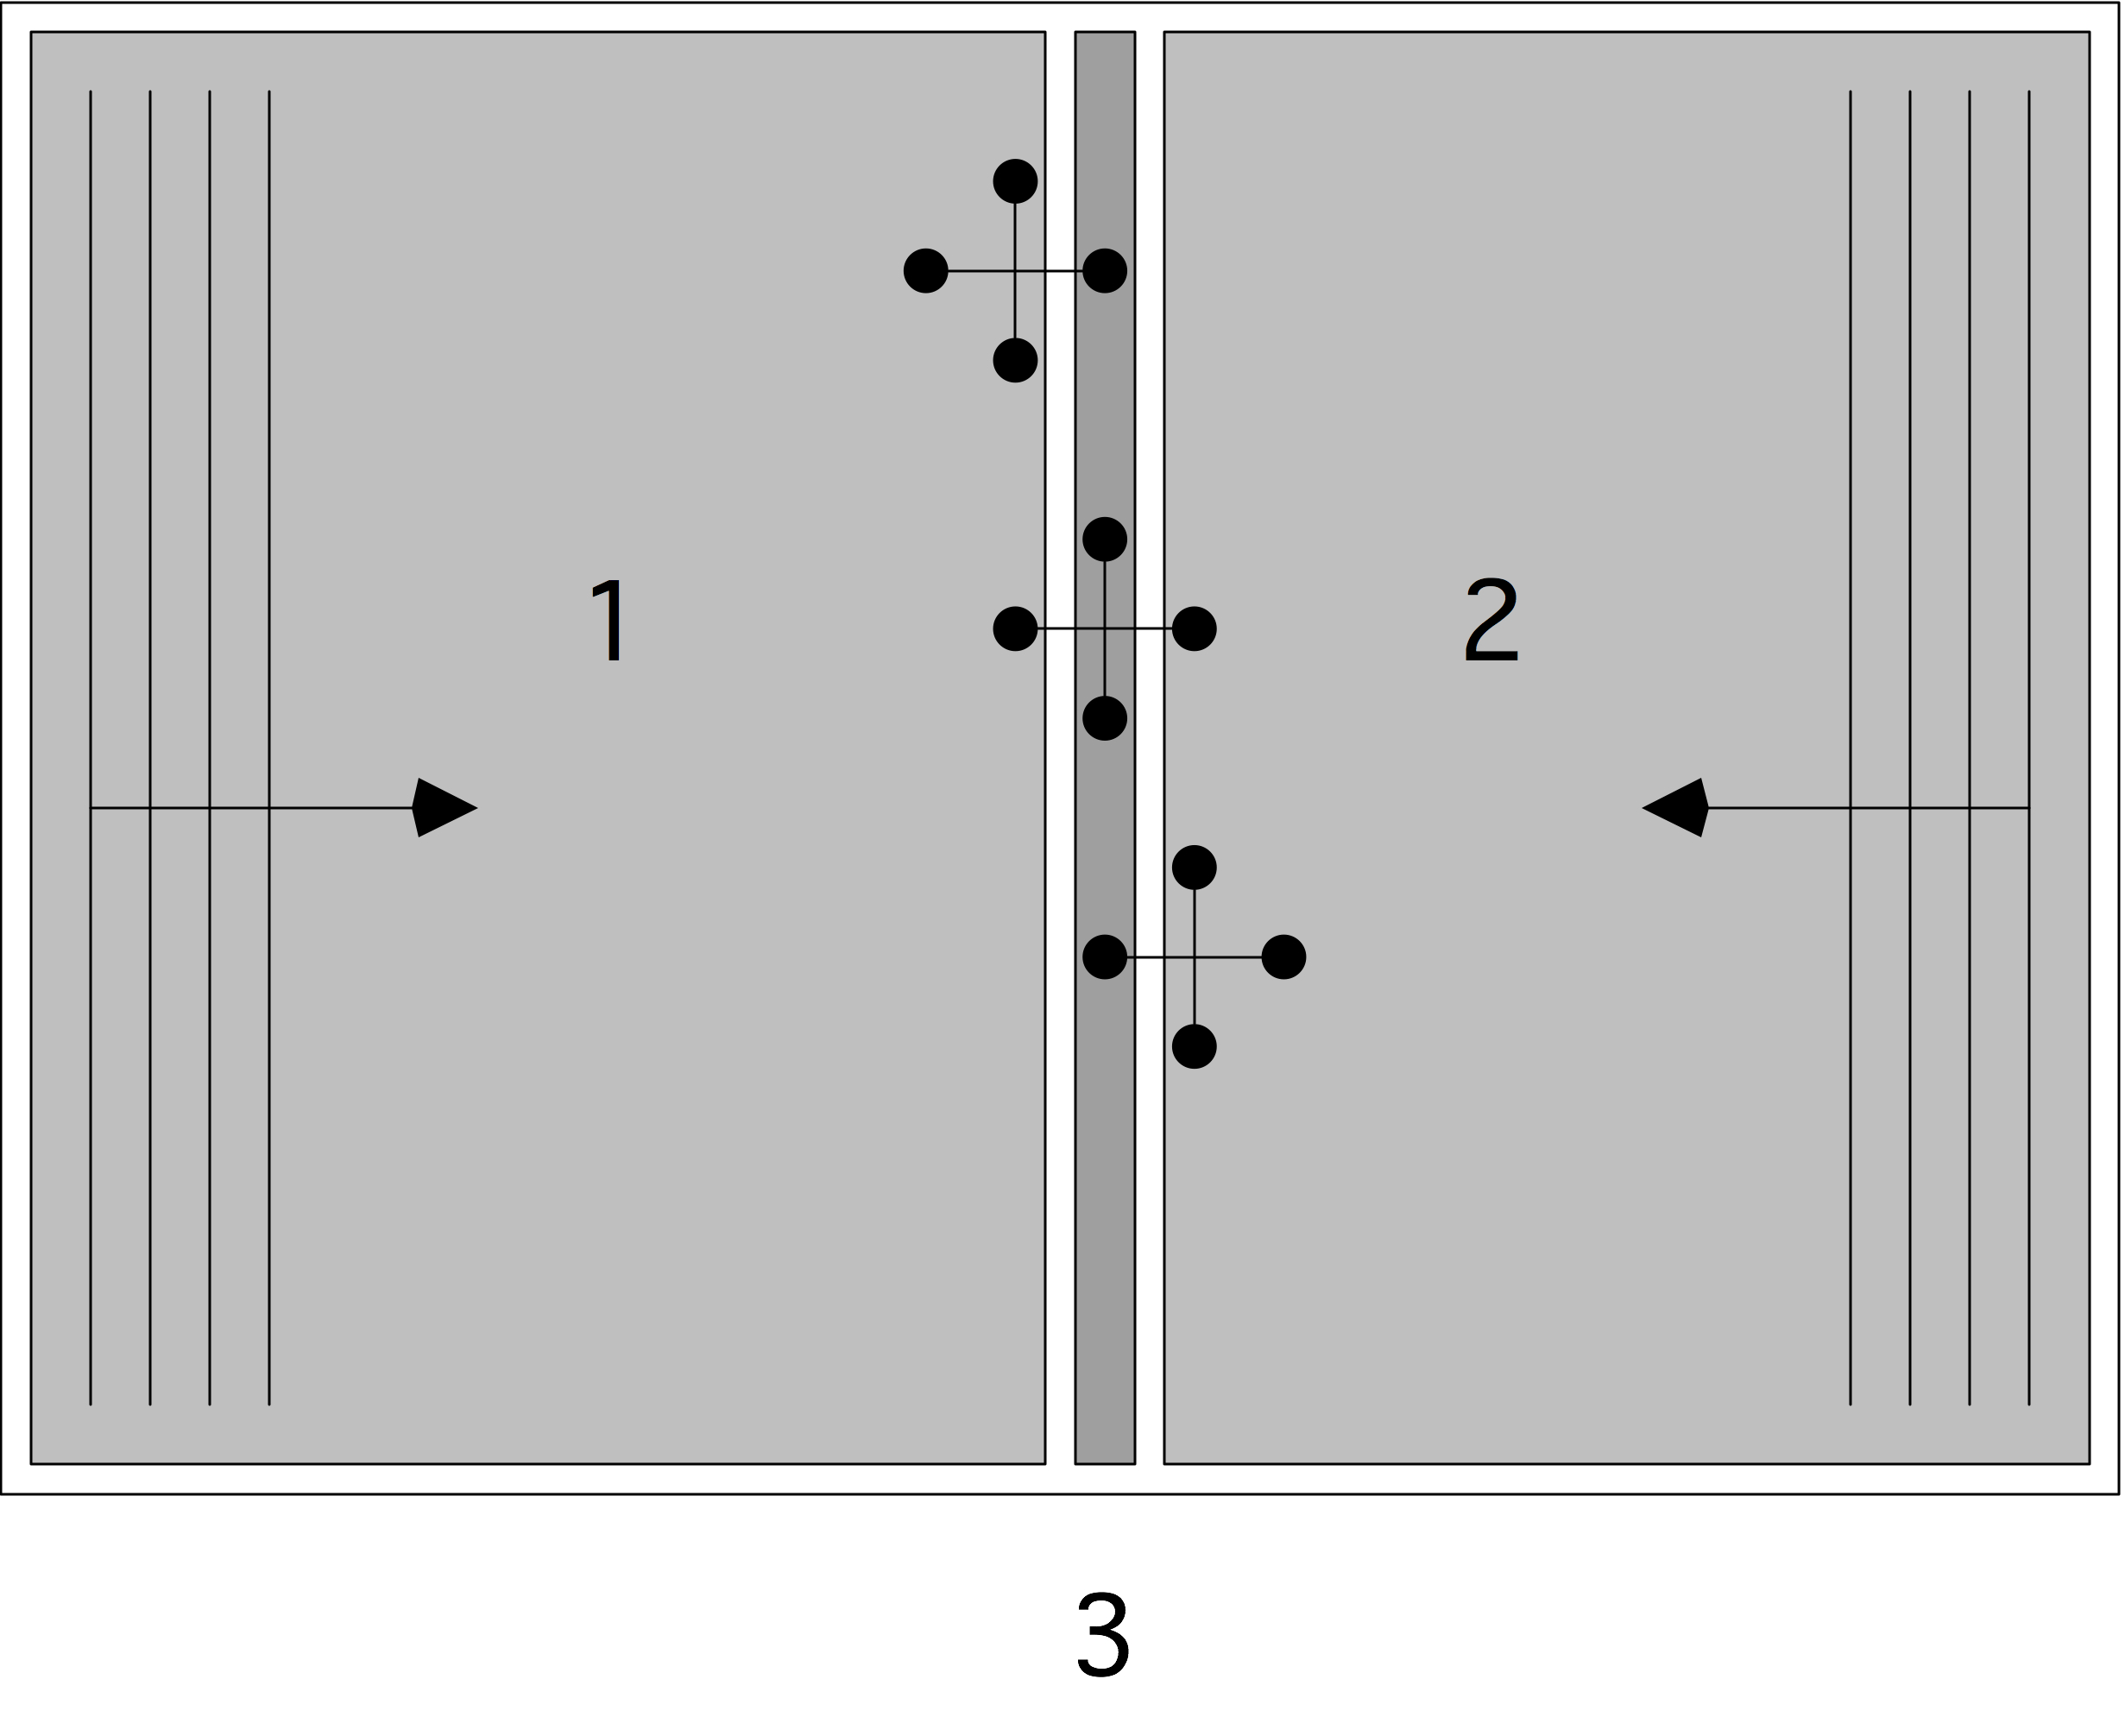
\includegraphics[scale=.1]{graphics/domdecomp}
}

\newcommand\Add{A^{\mathrm{DD}}}

\frame{\small
\[
\left(\begin{array}{ccccc|ccccc|c}
  \star&\star &      &      &      &&&&&&0\\
  \star&\star &\star &      &      &&&&&&\vdots\\
       &\ddots&\ddots&\ddots&      &&&\emptyset&&&\vdots\\
       &      &\star &\star &\star &&&&&&0\\
       &      &      &\star &\star &&&&&&\star\\ \hline
  &&&&&\star&\star &      &      &      &0\\
  &&&&&\star&\star &\star &      &      &\vdots\\
  &&\emptyset&&&     &\ddots&\ddots&\ddots&      &\vdots\\
  &&&&&     &      &\star &\star &\star &0\\
  &&&&&     &      &      &\star &\star &\star\\ \hline
  0&\cdots&\cdots&0&\star&0&\cdots&\cdots&0&\star&\star
\end{array}\right)
\begin{array}{c}
  \left.\begin{array}{c}
    \phantom{x}\\ \phantom{x}\\ \phantom{x}\\ \phantom{x}\\ \phantom{x}\\
  \end{array}\right\} \\
  \left.\begin{array}{c}
    \phantom{x}\\ \phantom{x}\\ \phantom{x}\\ \phantom{x}\\ \phantom{x}\\
  \end{array}\right\} \\
  \left.\begin{array}{c}
    \phantom{x}\\ 
  \end{array}\right\}
\end{array}
\begin{array}{c}
  \phantom{x}\\ \phantom{x}\\ (n^2-n)/2\\ \phantom{x}\\ \phantom{x}\\
  \phantom{x}\\ \phantom{x}\\ (n^2-n)/2\\ \phantom{x}\\ \phantom{x}\\
  n
\end{array}
\]
}

\frame{\frametitle{DD factorization}

\[
\begin{array}{l}
\Add=
  \begin{pmatrix}
    A_{11}&\emptyset&A_{13}\\
    \emptyset&A_{22}&A_{23}\\
    A_{31}&A_{32}&A_{33}
  \end{pmatrix}=\\[10pt]
  \begin{pmatrix}
    I\\
    \emptyset&I\\
    A_{31}A_{11}\inv&A_{32}A_{22}\inv&I
  \end{pmatrix}
  \begin{pmatrix}
    A_{11}&\emptyset&A_{13}\\
         &A_{22}&A_{23}\\
    &&S
  \end{pmatrix}
\end{array}
\]
\[ S = A_{33}-A_{31}A_{11}\inv A_{13}-A_{32}A_{22}\inv A_{23} \]
Parallelism\ldots
}

\frame{\frametitle{Graph theory of sparse elimination}
\only<1,3>{
\[ a_{ij} \leftarrow a_{ij}- a_{ik}a_{kk}\inv a_{kj} \]
  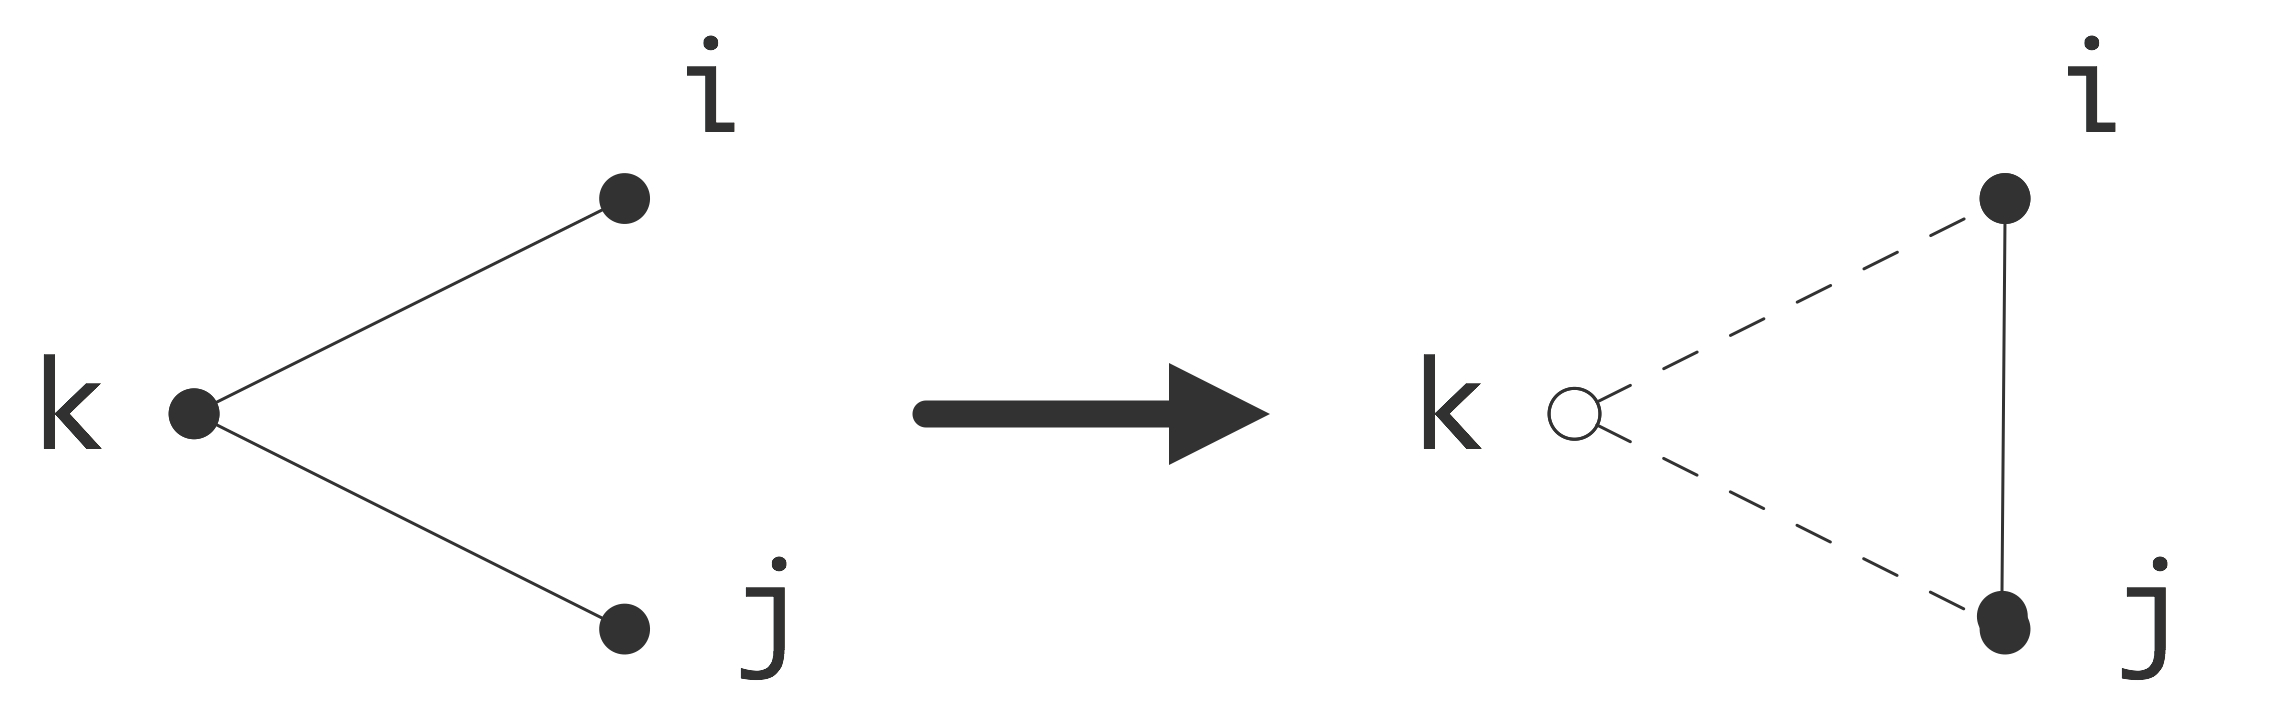
\includegraphics[scale=.12]{graphics/ijk-eliminate}
}

\only<2>{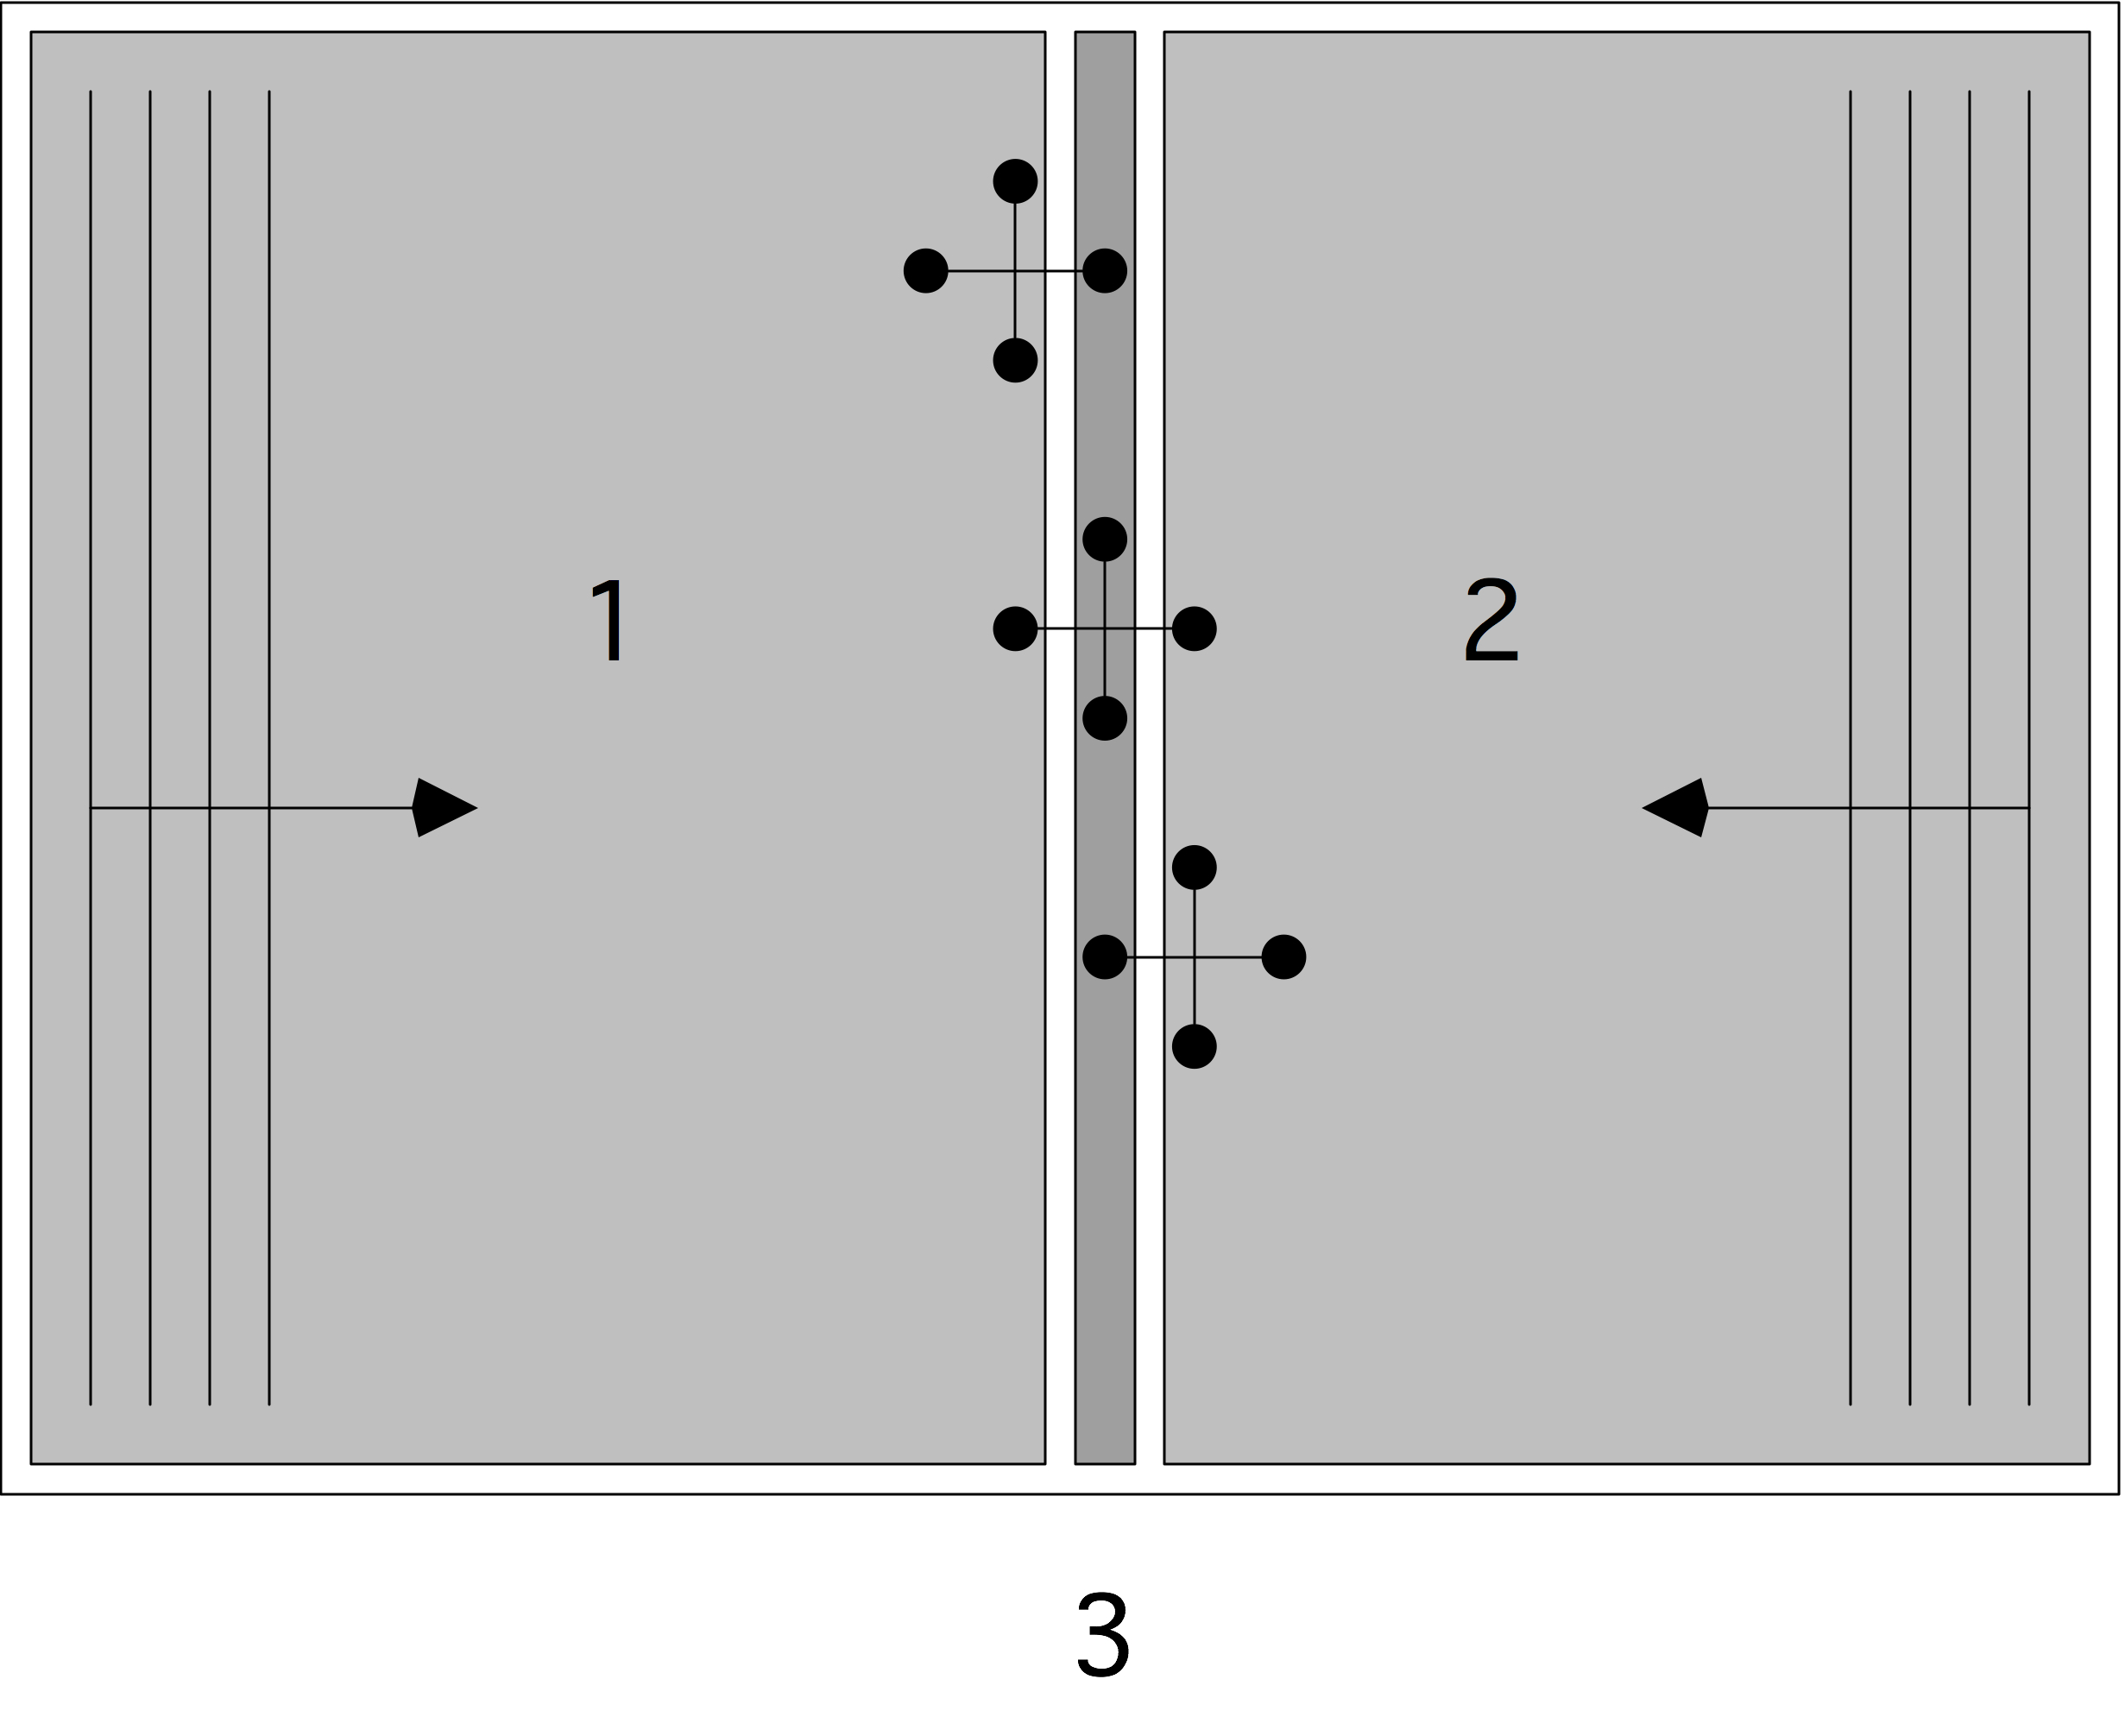
\includegraphics[scale=.08]{graphics/domdecomp}}

\only<3->{So inductively $S$ is dense}
}

\frame{\frametitle{Recursive bisection}
\begin{figure}
  \begin{quote}
    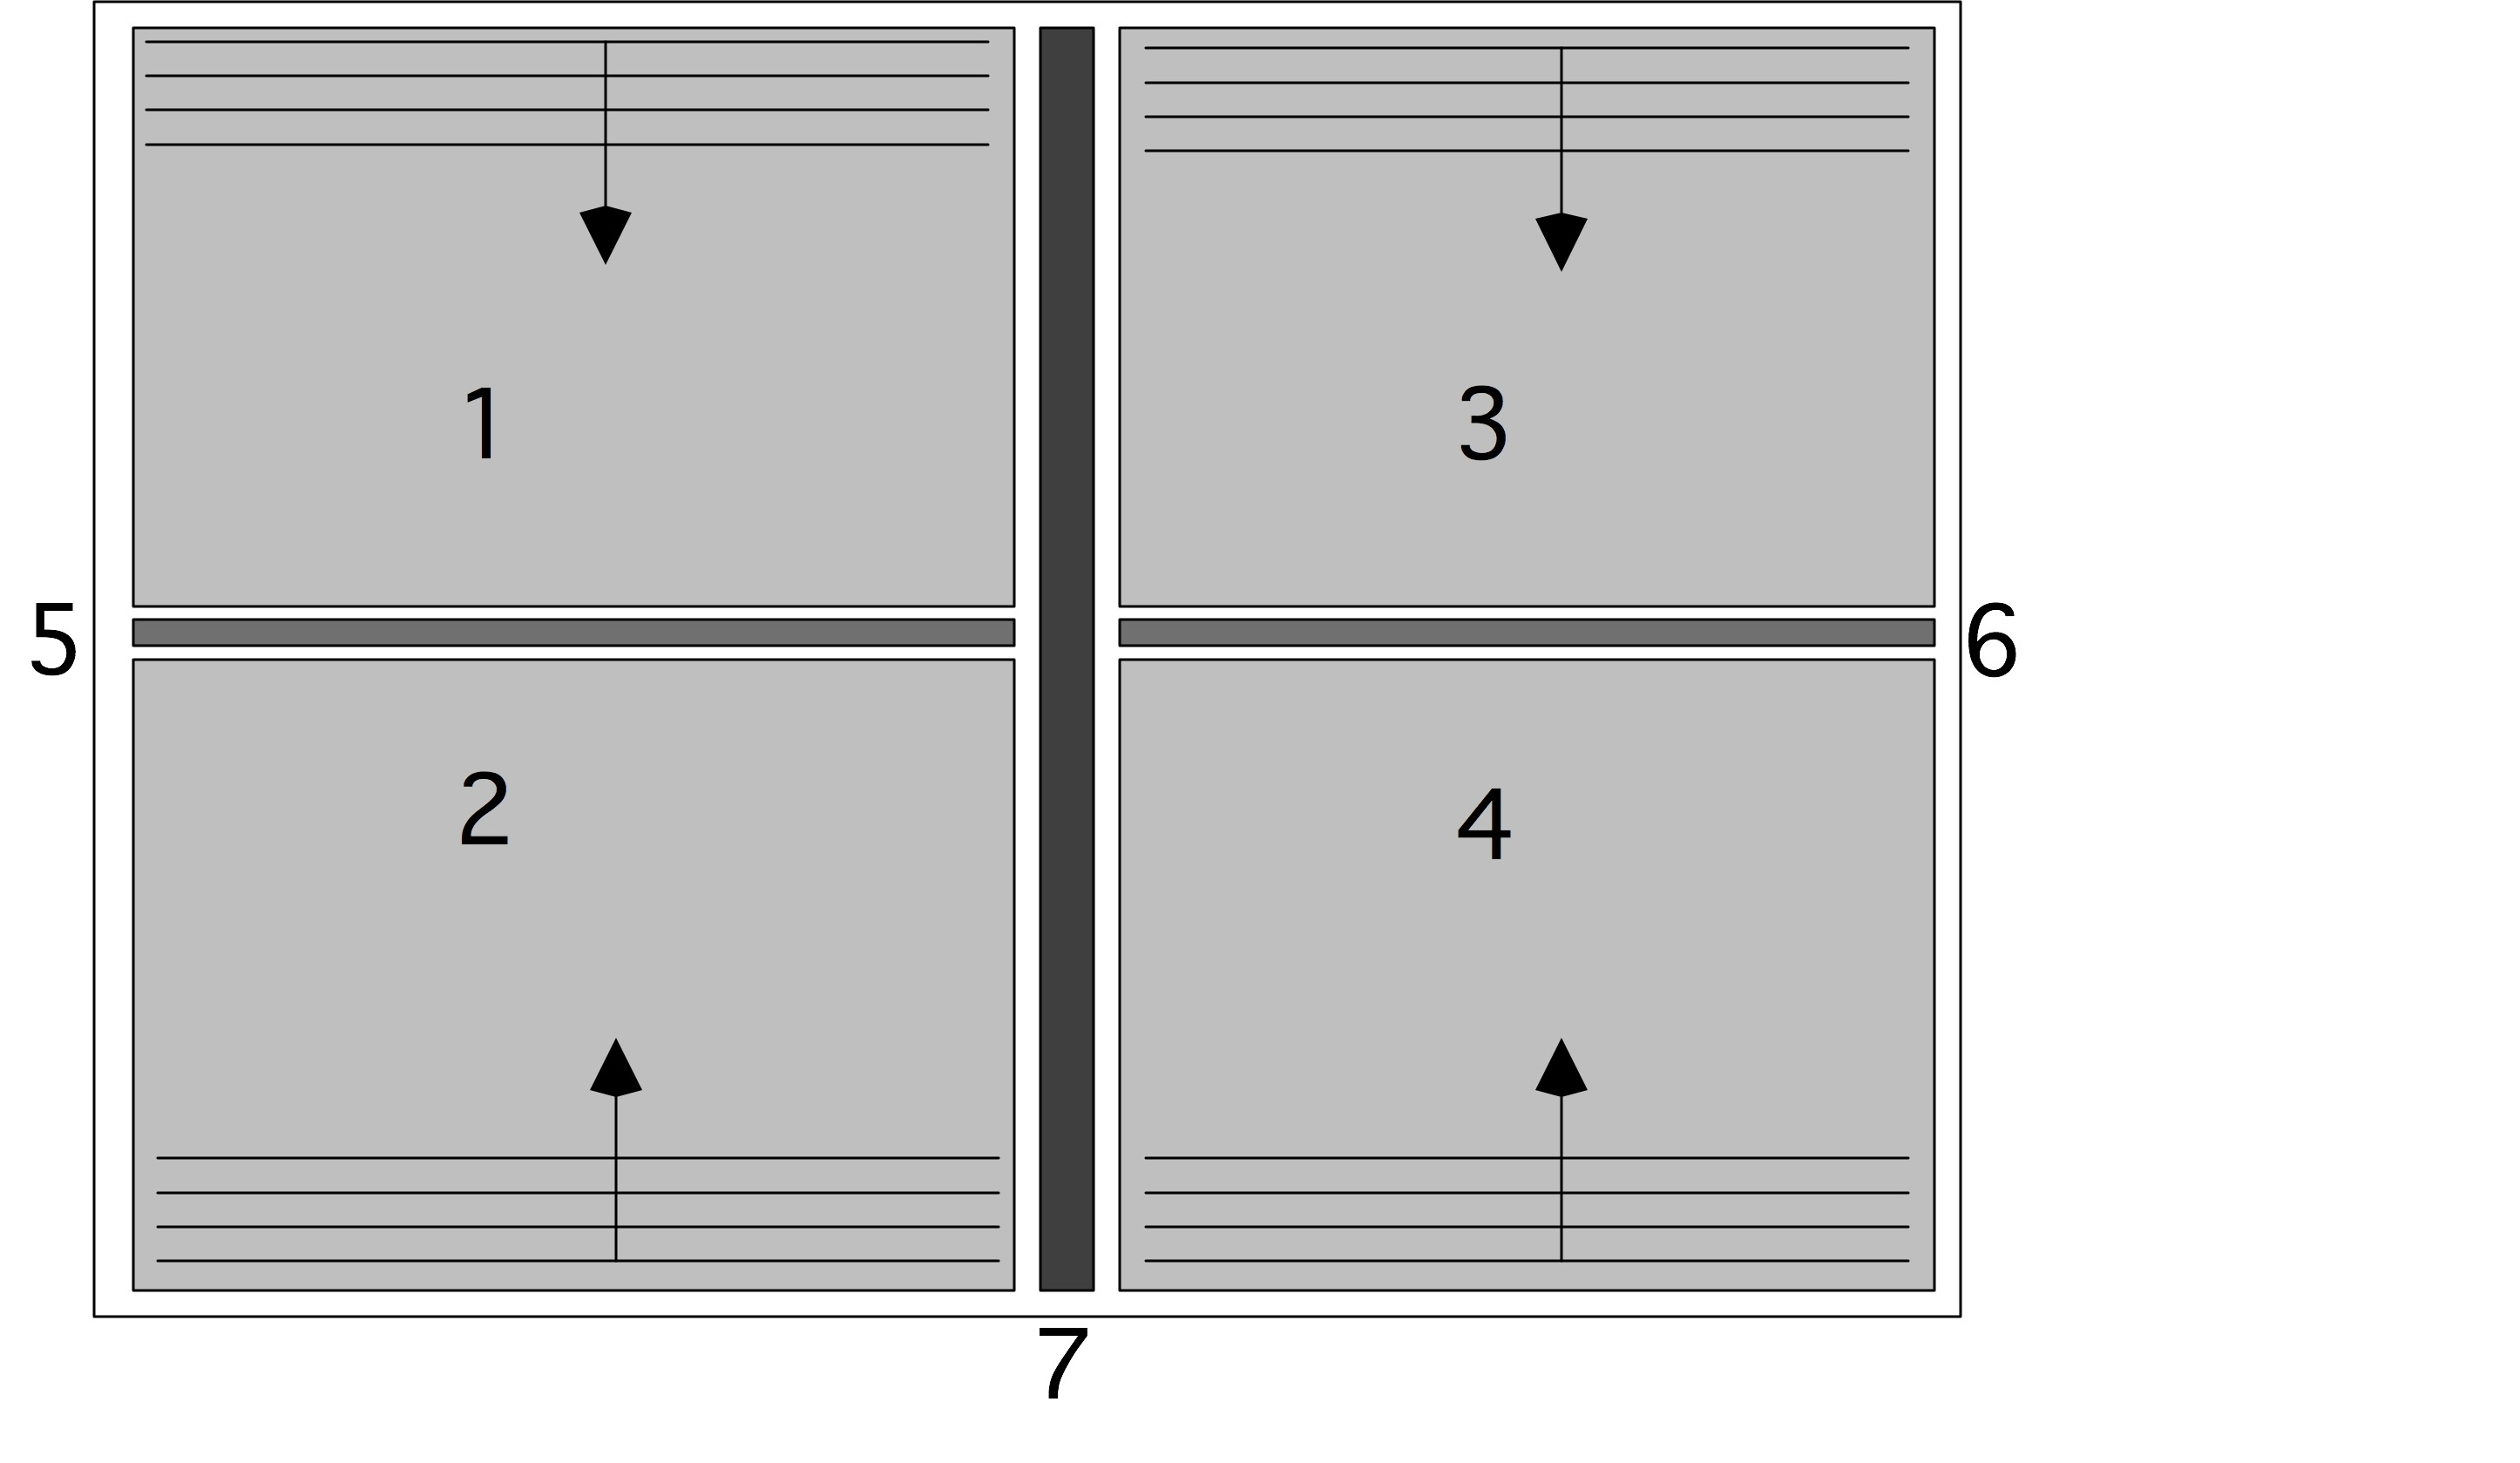
\includegraphics[scale=.11]{graphics/domdecomp2}
  \end{quote}
  \caption{A four-way domain decomposition}
  \label{fig:domdecomp2}
\end{figure}
}
\frame{
\[
  \Add=
  \left(\begin{array}{ccccccc}
    A_{11}&     &     &     &A_{15}&     &A_{17}\\
         &A_{22}&     &     &A_{25}&     &A_{27}\\
         &     &A_{33}&     &     &A_{36}&A_{37}\\
         &     &     &A_{44}&     &A_{46}&A_{47}\\ 
    A_{51}&A_{52}&    &     &A_{55}&      &A_{57}\\
         &      &A_{63}&A_{64}&    &A_{66}&A_{67}\\
    A_{71}&A_{72}&A_{73}&A_{74}&A_{75}&A_{76}&A_{77}
  \end{array}\right)
\]
The domain/operator/graph view is more insightful, don't you think?
}

\frame{\frametitle{How does this look in reality?}
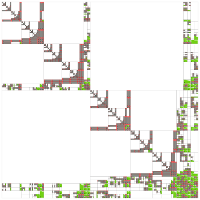
\includegraphics[scale=2.5]{graphics/nesteddis}
}

\frame{\frametitle{Fill-in is a function of ordering}

  \[ 
  \begin{pmatrix}
    *&*&\cdots&*\\ *&*&&\emptyset\\ \vdots&&\ddots\\ *&\emptyset&&*
  \end{pmatrix}
  \]
  After factorization the matrix is dense.\\
  Can this be permuted?
}

\frame{\frametitle{Fill-in during LU}

Fill-in: index $(i,j)$ where $a_{ij}=0$ but $\ell_{ij}\not=0$ or
$u_{ij}\not=0$.

2D BVP: $\Omega$ is $n\times n$, gives matrix of size $N=n^2$, with
bandwidth~$n$. 

Matrix storage $O(N)$

LU storage $O(N^{3/2})$

LU factorization work $O(N^2)$

Without proof: nested dissection $O(N\log N)$ space, $O(N^{3/2})$ work
}

\sectionframe{Parallel preconditioners}

\frame[containsverbatim]{\frametitle{Sparse operations in parallel: mvp}
Mvp $y=Ax$
\begin{verbatim}
  for i=1..n
    y[i] = sum over j=1..n a[i,j]*x[j]
\end{verbatim}
In parallel:
\begin{verbatim}
  for i=myfirstrow..mylastrow
    y[i] = sum over j=1..n a[i,j]*x[j]
\end{verbatim}
}

\frame[containsverbatim]{\frametitle{How about ILU solve?}
Consider $Lx=y$
\begin{verbatim}
  for i=1..n
    x[i] = (y[i] - sum over j=1..i-1 ell[i,j]*x[j]) 
           / a[i,i]
\end{verbatim}
Parallel code:
\begin{verbatim}
  for i=myfirstrow..mylastrow
    x[i] = (y[i] - sum over j=1..i-1 ell[i,j]*x[j]) 
           / a[i,i]
\end{verbatim}
Problems?
}

\frame[containsverbatim]{\frametitle{Block method}
\begin{verbatim}
  for i=myfirstrow..mylastrow
    x[i] = (y[i] - sum over j=myfirstrow..i-1 ell[i,j]*x[j]) 
           / a[i,i]
\end{verbatim}
Block Jacobi with local GS solve
}

\frame{\frametitle{}
\begin{figure}[ht]
  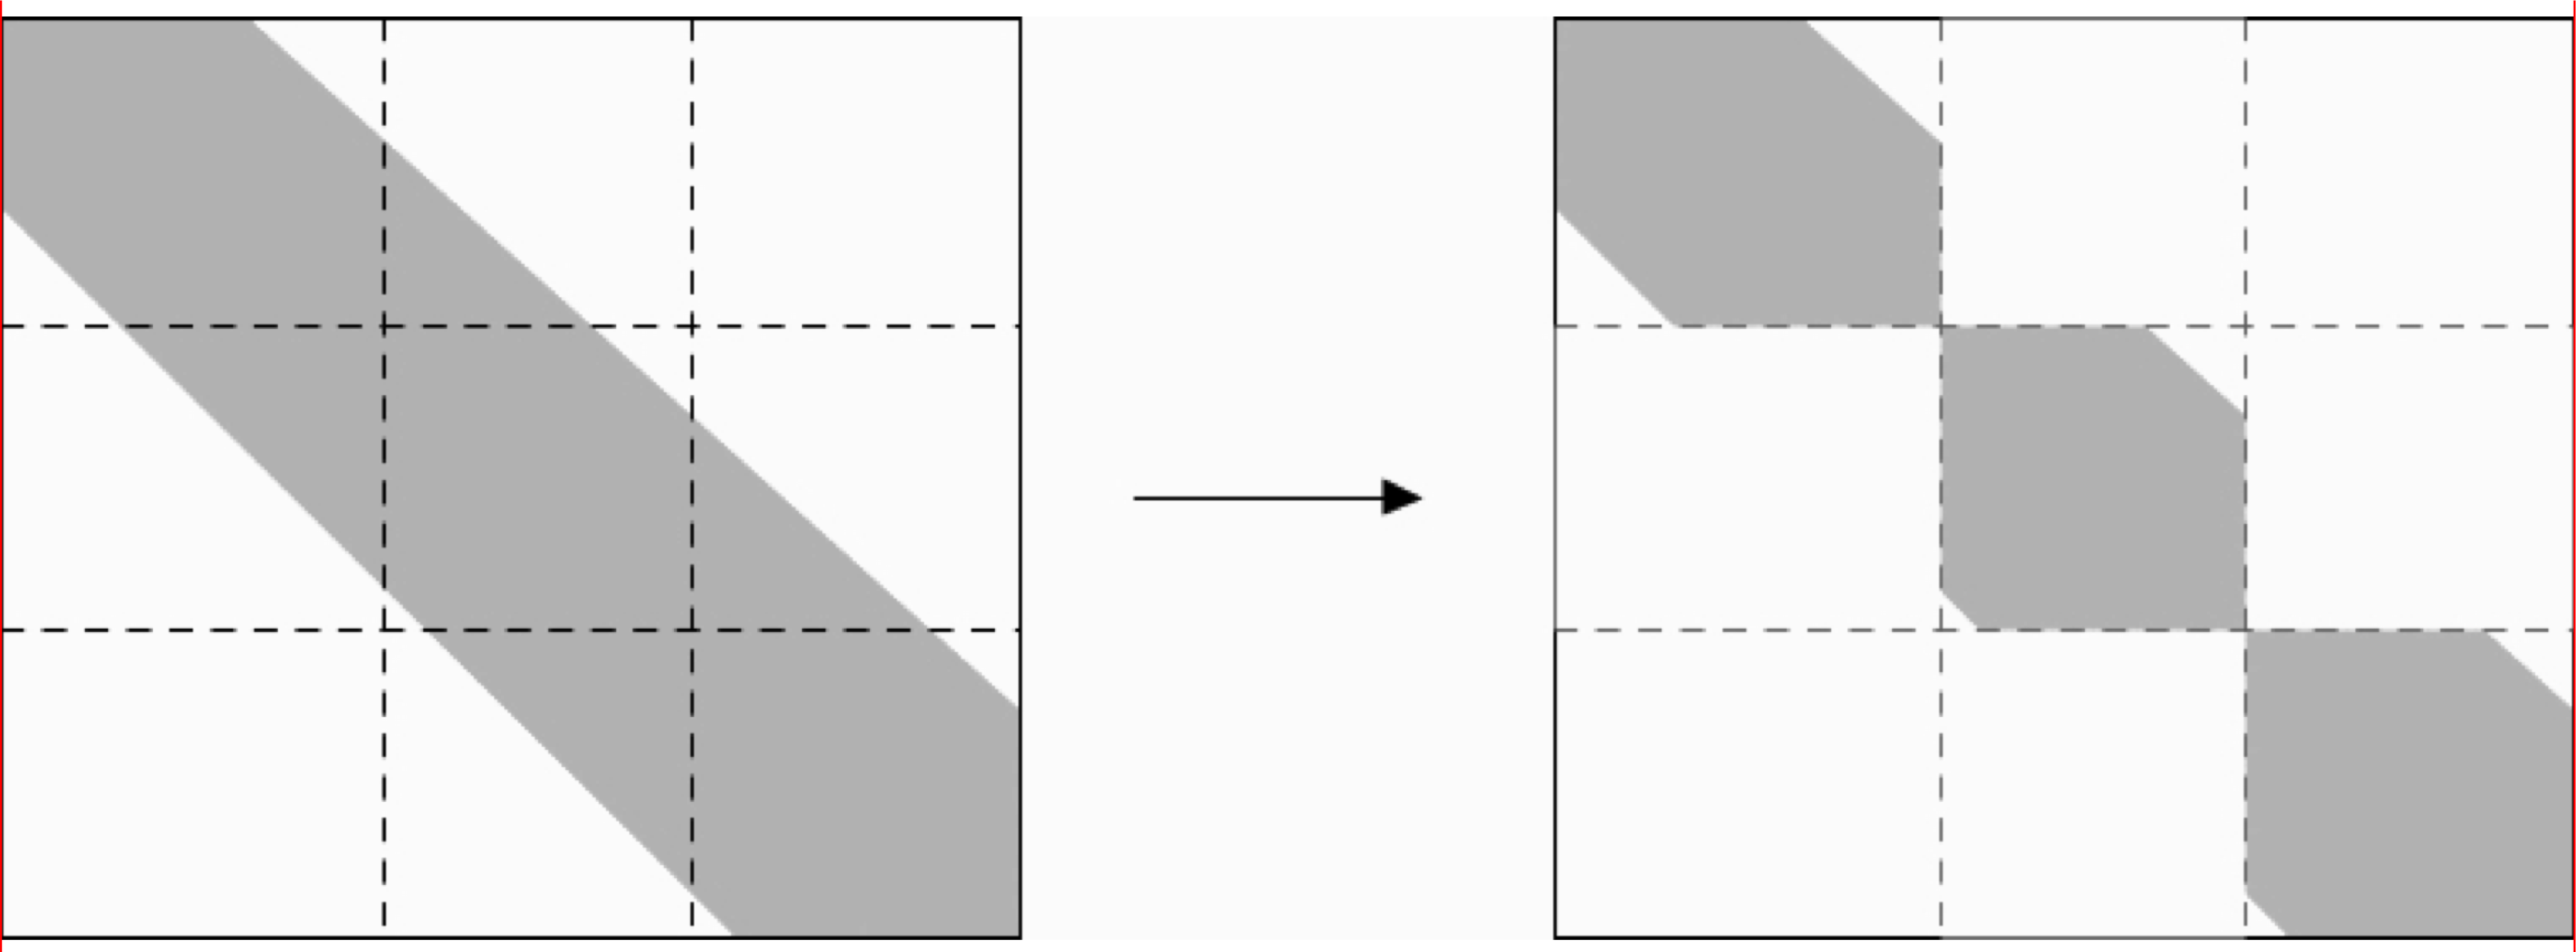
\includegraphics[scale=.12]{graphics/block-jacobipdf}
  \caption{Sparsity pattern corresponding to a block Jacobi
    preconditioner}
  \label{fig:block-method}
\end{figure}
}

\frame{\frametitle{Multicolour ILU}
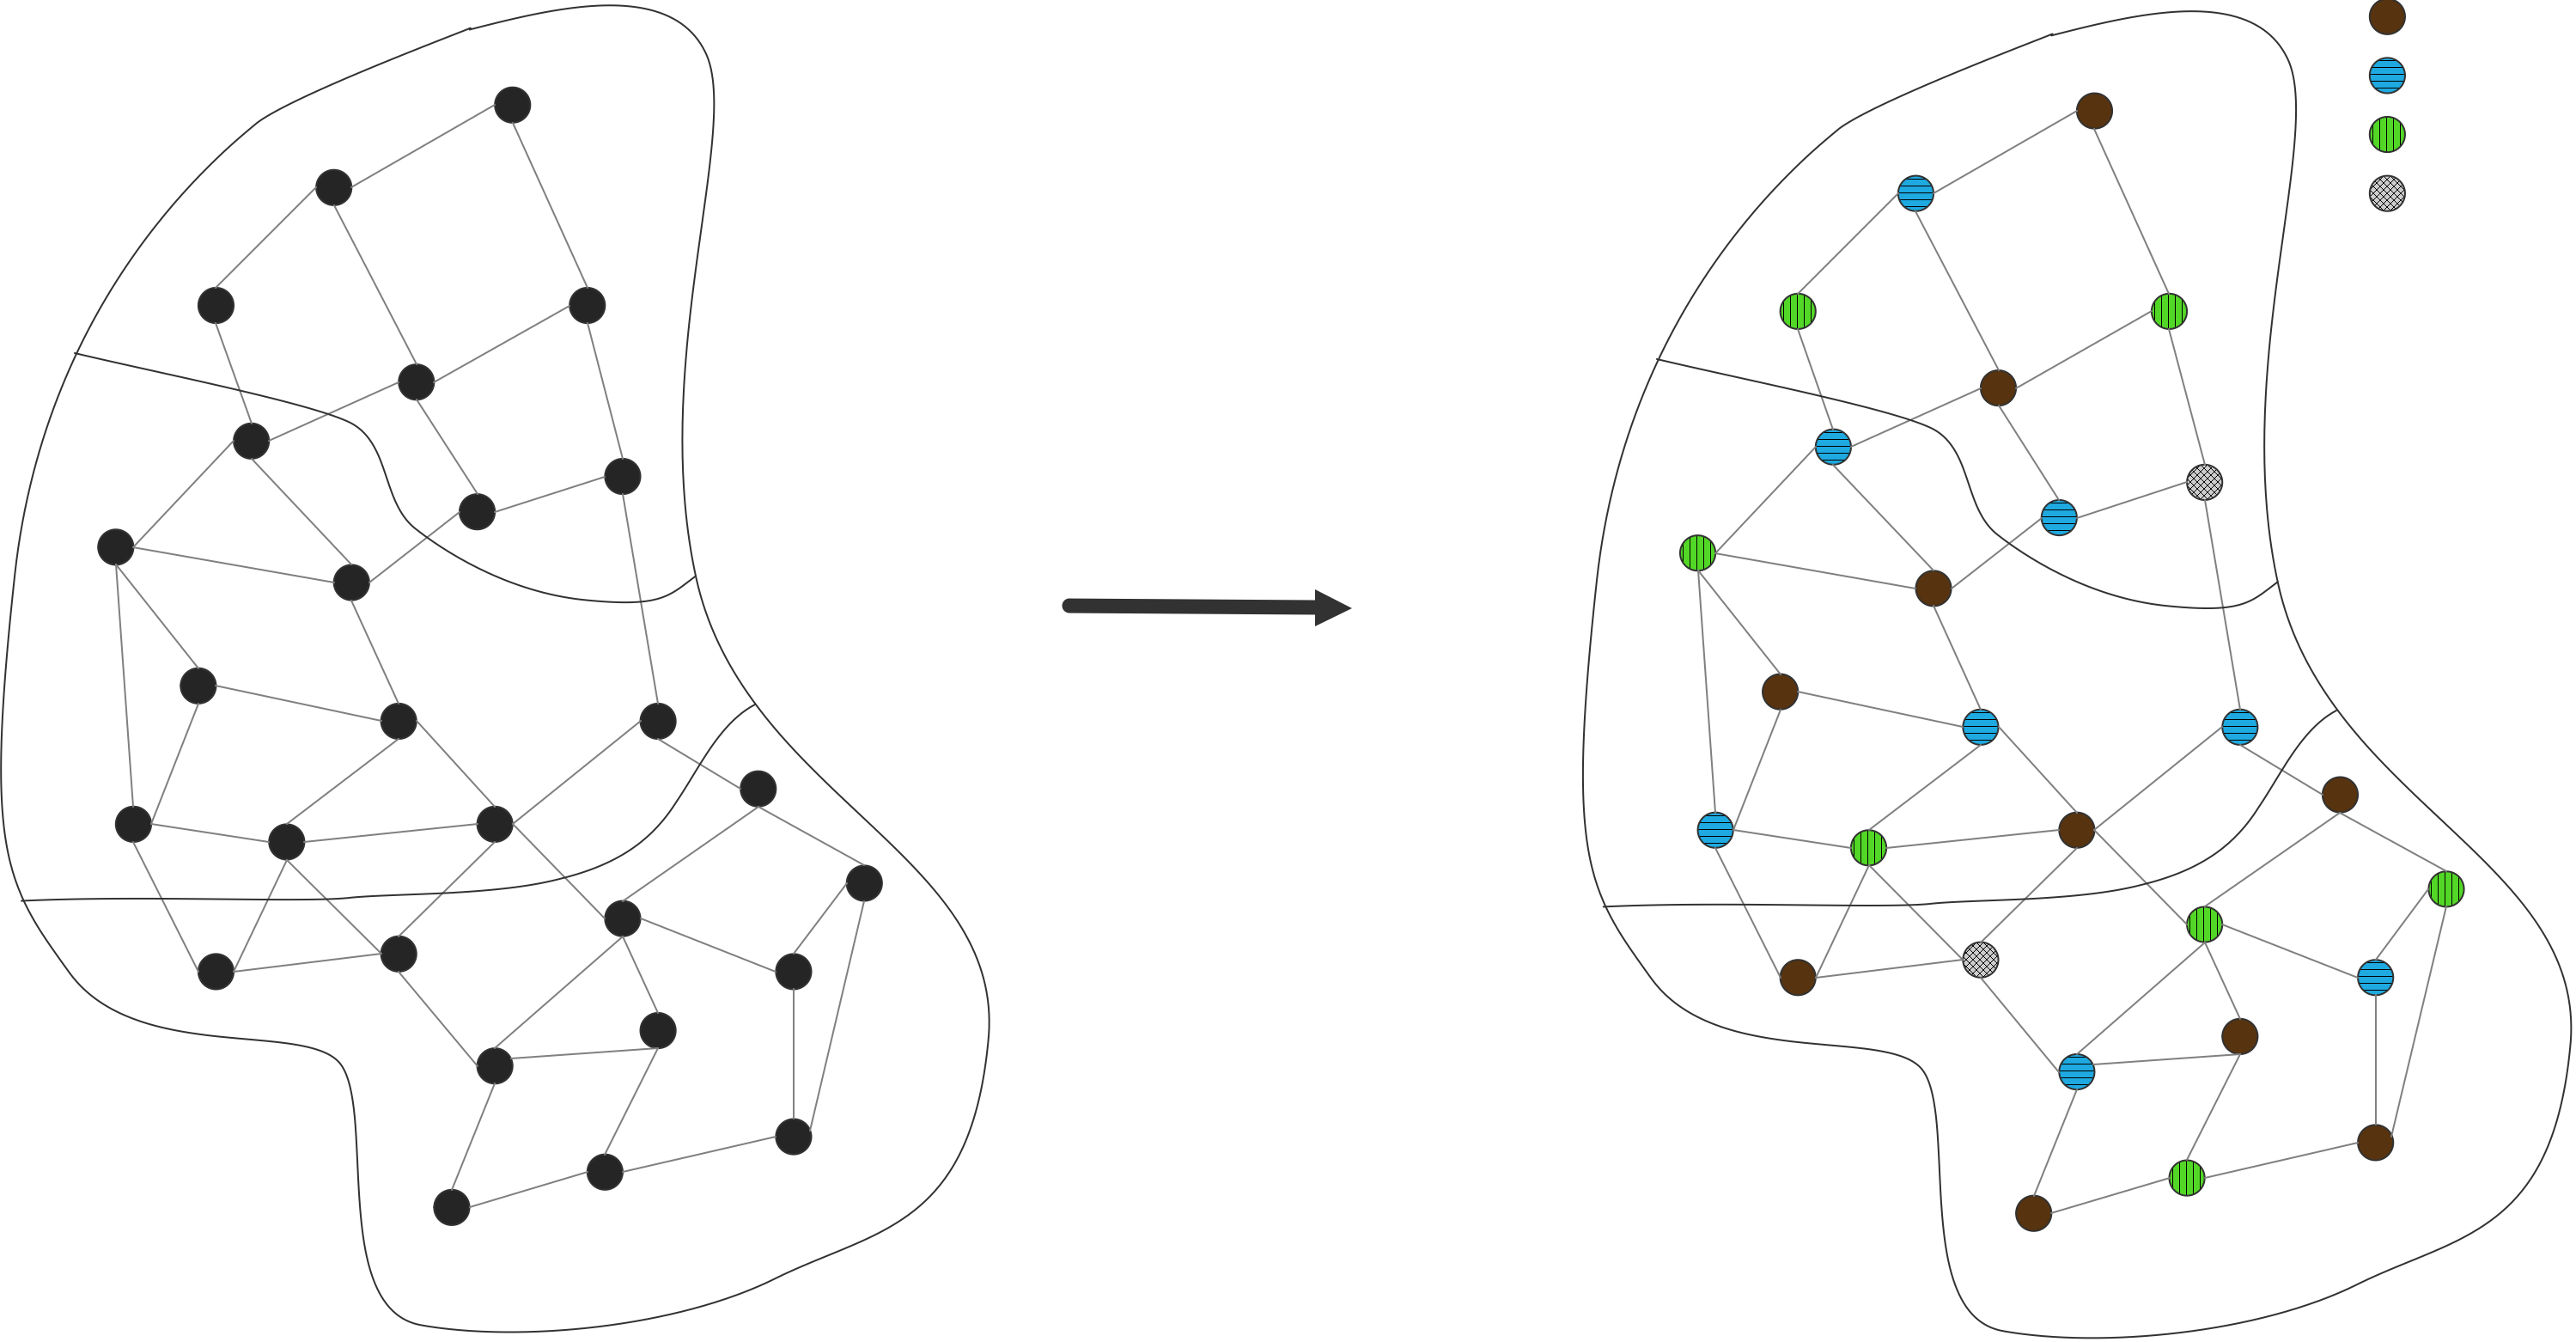
\includegraphics[scale=.1]{graphics/pilu}
}
\frame{\frametitle{}
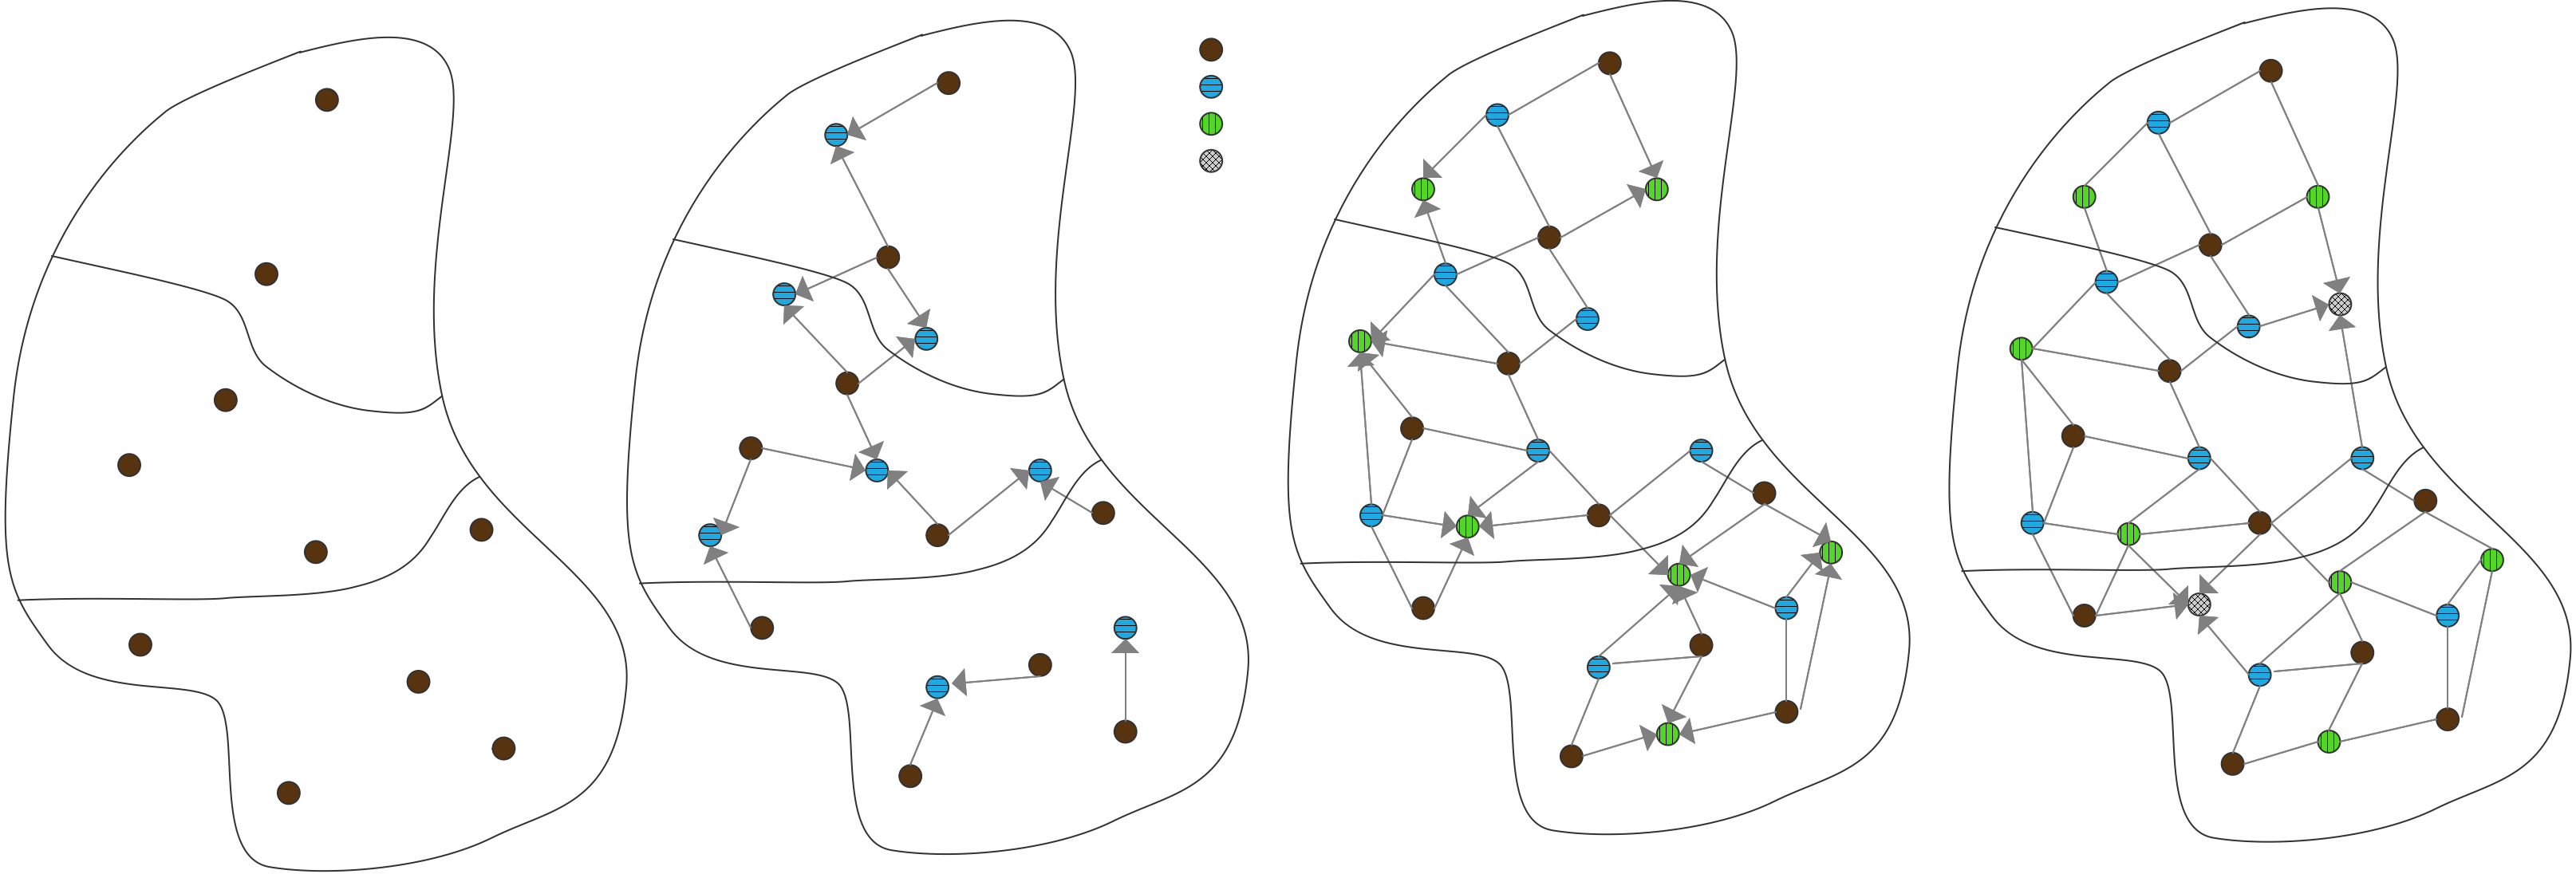
\includegraphics[scale=.1]{graphics/pilu-solve}
}

\end{document}

\frame{\frametitle{Variable reordering}
\footnotesize
\[ 
\begin{pmatrix}
  a_{11}&a_{12}&&&&\emptyset\\ a_{21}&a_{22}&a_{23}\\ 
  &a_{32}&a_{33}&a_{34}\\ \emptyset&&\ddots&\ddots&\ddots
\end{pmatrix}
\begin{pmatrix}  x_1\\ x_2\\ x_3\\ \vdots\end{pmatrix} =
\begin{pmatrix}  y_1\\ y_2\\ y_3\\ \vdots\end{pmatrix}
\]
with redblack
\[ 
\begin{pmatrix}
  a_{11}&&&&a_{12}\\ &a_{33}&&&a_{32}&a_{34}\\ &&a_{55}&&&\ddots&\ddots\\
  &&&\ddots\\
  a_{21}&a_{23}&&&a_{22}\\ &a_{43}&a_{45}&&&a_{44}\\ &&\ddots&\ddots&&&\ddots
\end{pmatrix}
\begin{pmatrix}  x_1\\ x_3\\ x_5\\ \vdots\\ x_2\\ x_4\\ \vdots\end{pmatrix} =
\begin{pmatrix}  y_1\\ y_3\\ y_5\\ \vdots\\ y_2\\ y_4\\ \vdots\end{pmatrix}
\]
Two-processor parallel Gauss-Seidel or ILU
}

\frame{\frametitle{2D redblack}
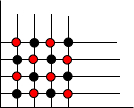
\includegraphics{graphics/redblack}

In general, colouring, colour number
}

\frame{\frametitle{Turning implicit operations into explicit}
Normalize ILU solve to $(I-L)$ and $(I-U)$

Approximate $(I-L)x = y$ by $x\approx (I+L+L^2)y$

Convergence guaranteed for diagonally dominant
}


\frame{\frametitle{}
}

\frame{\frametitle{}
}


\end{document}
